%!TEX root = ../../diss.tex
\chapter[Foundations]{Foundations}\label{chap:rw:passwords}
%lingo: adversaries statt attackers, a-priory knowledge

% general broad description of where passwords play a role and what authentication is.
Passwords are but one puzzle piece in the realm of cyber security. They are part of the access control paradigm, which is commonly divided into three steps: identification, authentication, and authorization \cite{Riley2006IdentityAuthenticationDistinct}. Identifying a user is usually done with a prompt for a user name, so the system tries to answer the question ``who are you?''. Authentication is about proving that a user -- or more broadly an entity -- is who they claim to be, i.e. authentication is about verification of an identified entity. In other words, the system asks ``How can you prove that you are who you claim to be?''. This verification process can be based on three central elements, namely something that you know (any kind of secret), something that you are (any kind of property), or something that you have (any kind of secret token). One could argue that the second category could be extended by ``something that you do?'', e.g. provide your individual signature. However, authentication does not necessarily \textit{require} identification as a first step. It is well possible to authenticate entities even if they are anonymous. One everyday example are passwords for WiFi networks: Most of the time, the access point does not require a user name; the password, or pre-shared key, in a \gls{WPA} protocol is enough to join the network. 
Last, authorization is the decision over which resources an authenticated entity is allowed to use, or an answer to ``can the user access this?''.


For this thesis, \textbf{authentication} remains the center of attention. In this chapter, we take a look at various forms of authentication and establish an argument as to why ``something that you know'' is still the most prevalent and significant authentication paradigm to date. 

\section{A Brief History of Passwords}
% first passwords were those on CTSS
The idea of protecting resources with ``something that you know'' is hundreds of years old. Think about the magic words ``open, Sesame!'' that Ali Baba spoke to enter a den used as treasury by forty thieves\footnote{Ali Baba is a fictional character in a story from ``Thousand and One Nights'' as recorded by Antoine Galland in the early 18th century. \url{http://www.pitt.edu/~dash/alibaba.html} \la{16.12.2017}}. The story already illustrates password misuse, because Ali Baba was not the rightful owner of the den and he impersonated the thieves. Nonetheless, this authentication paradigm was brought to the digital world in the early 1960s by the Massachusetts Institute of Technology (MIT) \footnote{\url{https://www.wired.com/2012/01/computer-password/}, \access{16.12.2017}}. Researchers had built a mainframe computer that was programmable by multiple users. At the time, one of the most valuable resources beside the physical device was the \textit{time} granted to use the machine. Thus, the Compatible Time Sharing System (CTSS) was conceived to give every user a certain quota of hours to operate the computer. The quota was enforced by creating user accounts that were password protected. The interaction very much resembles what we still use today: after typing the user name, the password is requested and hidden from the screen during entry.


% First flaws were evident, when the first attack happened
Shortly afterwards, the flaws of the system started to become evident when Alan Scherr became the first ``hacker''\footnote{\url{https://www.slideshare.net/CAinc/history-of-the-password/7-In_1962_a_software_bug} \la{16.12.2017}}. He desired more usage time, so he needed to impersonate other users of the computer and use their quota. The list of passwords on the system was not well protected, which allowed him to access the credentials and carry out what was probably the first password exploit in computer history. Scherr benefited from the fact that passwords were kept in plain text and could be accessed with a special punch card. Interestingly the attack was not detected immediately. Morris and Thompson mention strange behavior in their 1979 paper and blame the issue on a ``software design error'' \cite{Morris1979PasswordSecurity}, while in fact it was Scherr who was responsible for it\footurl{https://www.wired.com/2012/01/computer-password/}{05.03.2018}. 
% now we have crypto
With the rise of the UNIX operating system in the 1970s, encrypted passwords became standard. One of the cornerstones was the Data encryption standard (DES) which was developed by IBM and propagated by the US National Bureau of Standards (today called the National Institute of Standards and Technology, \gls{NIST}) \cite{Bishop1995ProactivePasswordChecking}. This algorithm was widely used until the late 1990s when computing power was sufficient to efficiently carry out attacks, which rendered DES infeasible. At the time, the Advanced Encryption Standard had already been proposed and was able to replace in a straightforward manner, so the issue was resolved quickly.%TODO could use a reference.  

%%%%%% TABLE BENEFITS AND DRAWBACKS OF PASSWORDS
% Table generated by Excel2LaTeX from sheet 'Sheet1'
\begin{table}[H]
  \centering
  \caption{\label{table:rw:benefits_drawbacks_pws}Benefits and Drawbacks for different stakeholders in a password-based authentication. SPs = service providers.}
  \resizebox{\linewidth}{!}{
    \begin{tabular}{llr}
	\cmidrule{1-3}    Stakes & \textbf{Benefits} & \multicolumn{1}{l}{\textbf{Drawbacks}} \\
	\cmidrule{1-3}    \rowcolor[rgb]{ .949,  .949,  .949} \textbf{SPs} & Low costs & \multicolumn{1}{l}{Large number of attack vectors} \\
	\rowcolor[rgb]{ .949,  .949,  .949}       & Easy to implement & \multicolumn{1}{l}{Anomaly detection costly} \\
	\rowcolor[rgb]{ .949,  .949,  .949}       & Replaceable when compromised & \multicolumn{1}{l}{Attacks are simple to carry out} \\
	\rowcolor[rgb]{ .949,  .949,  .949}       & Revocable by administrator & \multicolumn{1}{l}{Attack automation simple} \\
	\rowcolor[rgb]{ .949,  .949,  .949}       & Enforceable policies & \multicolumn{1}{l}{Attacks can have severe consequences} \\
	\rowcolor[rgb]{ .886,  .937,  .855} \textbf{Users} & Fast entry on desktops & \multicolumn{1}{l}{Memory overload from too many passwords} \\
	\rowcolor[rgb]{ .886,  .937,  .855}       & Most users already familiarized & \multicolumn{1}{l}{Suboptimal coping strategies} \\
	\rowcolor[rgb]{ .886,  .937,  .855}       & Easy to learn & \multicolumn{1}{l}{Stronger passwords difficult to memorize} \\
	\rowcolor[rgb]{ .886,  .937,  .855}       & Sharable with others & \multicolumn{1}{l}{Entry on mobile devices difficult} \\
	\rowcolor[rgb]{ .886,  .937,  .855}       & High degree of control / freedom & \multicolumn{1}{l}{Mastery difficult} \\
	\rowcolor[rgb]{ .886,  .937,  .855}       &       & \multicolumn{1}{l}{Disliked by many users / perceived as burden} \\
	\rowcolor[rgb]{ .851,  .882,  .949} \textbf{Misc} & Independent of identification & \multicolumn{1}{l}{Weak passwords are a risk for users and SPs } \\
	\rowcolor[rgb]{ .851,  .882,  .949}       & Adjustable security level &  \\
	\end{tabular}%
	}%end resizebox
\end{table}%
%%%%%% 

% we were happy with what we had on the system side, so we used it a lot especially on the web.
Around 50 years after CTSS, one of its creators, Fernando Corbató, said in an interview with the Wall Street Journal that password-based authentication has ``become kind of a nightmare with the World Wide Web''\footnote{\label{foot:corbato_regrets}\url{http://on.wsj.com/1sVQOIv}, \access{18.12.2017}}. The surge of the Web has lead to many services requiring authentication. Alphanumeric passwords were the go-to solution because the system is easy to implement and has almost no set-up costs other than a database. This has led to passwords becoming the de-facto standard for authenticating users on the Web.

% passwords do have drawbacks, which is why people have started to look into ways to replace them.
However, passwords do have shortcomings for all the stakeholders involved in the authentication process, e.g. users who struggle with remembering a multitude of passwords, or \glspl{SP} who need to deal with leaked passwords. Consequently, there have been many attempts to replace passwords as a whole to either minimize security risks, make things easier for the users, or -- ideally -- both at the same time. To this point, though, no alternative authentication mechanism has been able to fully replace alphanumeric passwords on the web, which we investigate in detail in Section \ref{sec:rw:authentication_without_pws}. Put short, the benefits provided by passwords outweigh the drawbacks most of the time. Table \ref{table:rw:benefits_drawbacks_pws} has a high-level overview of the benefits and drawbacks.


%more history in the introduction of \cite{Bishop1995ProactivePasswordChecking}, and of course as early as 1979 \cite{Morris1979PasswordSecurity}


\section{Attacks on Passwords}\label{sec:rw:attack_vectors}
As mentioned above, computer passwords were attacked shortly after they were called into action. Attacks have since become more sophisticated. In the first attack on passwords, Scherr benefited from very weak protection and was able to simply print the passwords and hack into the system. Nowadays, an attacker, or ``the bad guy'' as Morris and Thompson used to call them \cite{Morris1979PasswordSecurity}, has a number of ways to obtain a user's password(s). The following sections roughly depict how the attacks work, what the countermeasures look like, and if changing one's password behavior serves as effective countermeasure. 


%% Attack Overview Infographic
\begin{figure}[h!]
	\centering
	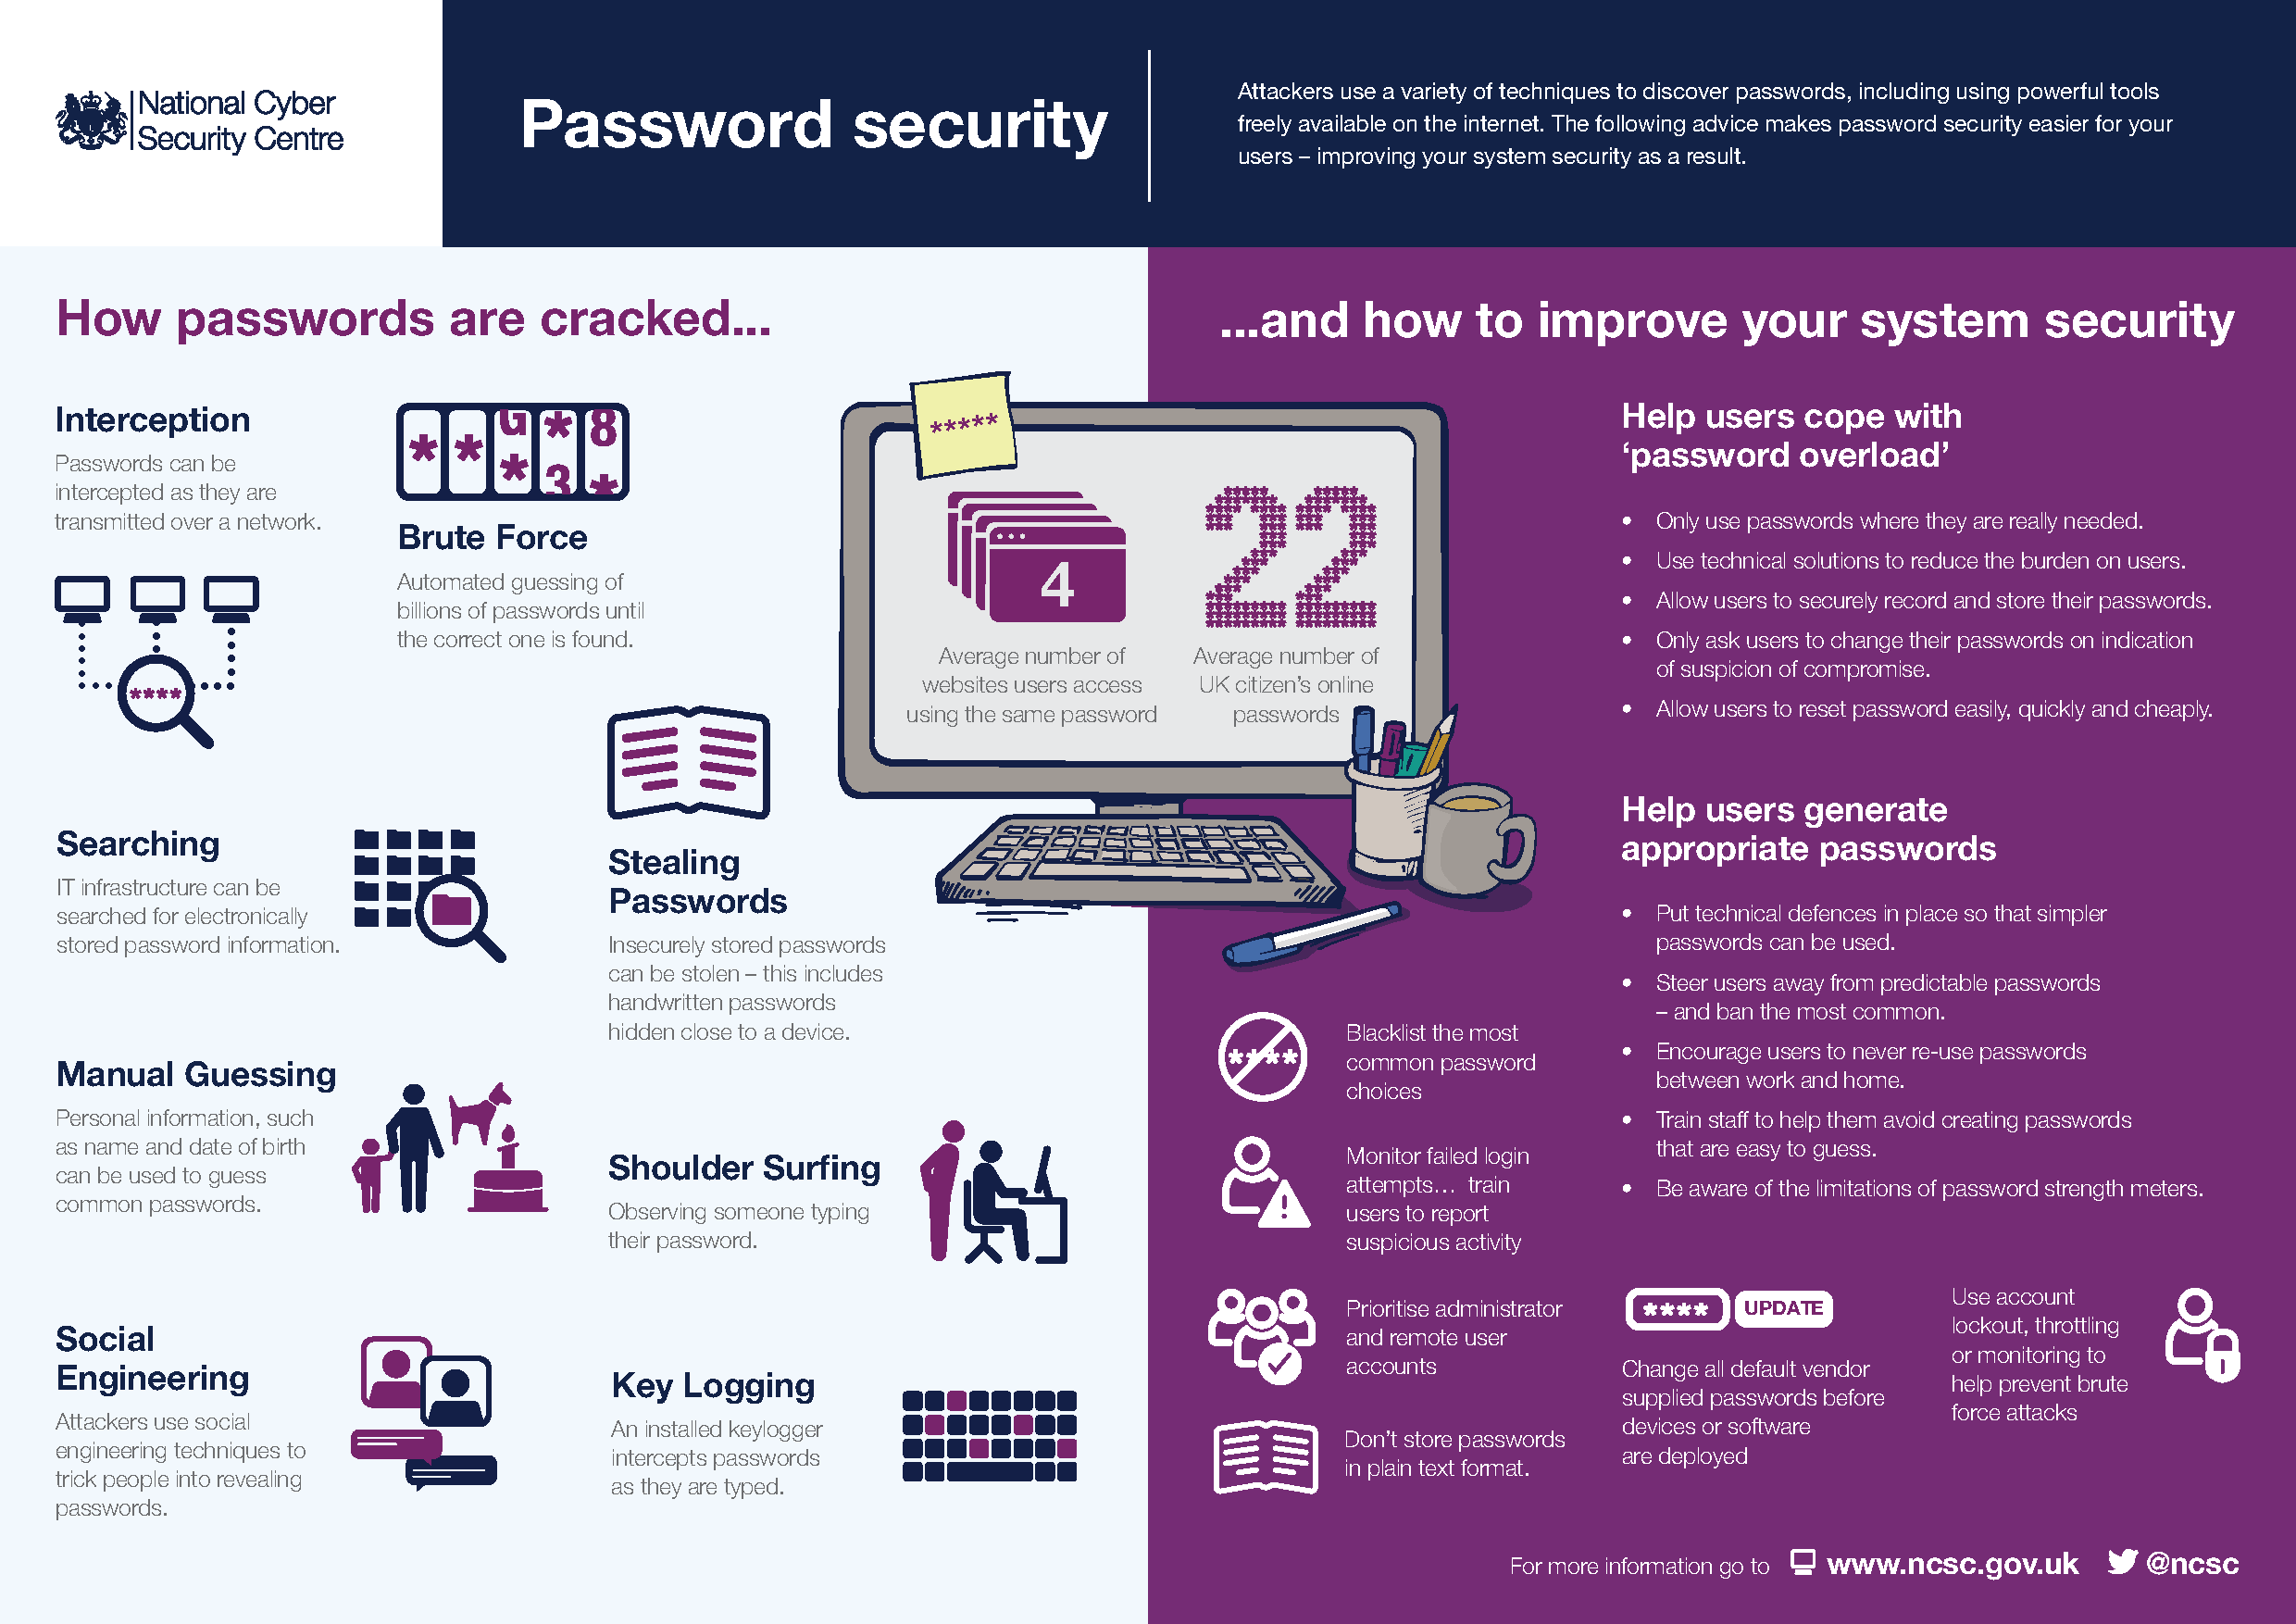
\includegraphics[width=\linewidth]{rw/NCSC-password-security-infographic}
	\caption{
		\label{fig:rw:attacks_infographic}
		Overview of attacks and high-level mitigations. Image courtesy of the National Cyber Security Centre, UK \protect\url{https://www.ncsc.gov.uk/guidance/password-collection} \protect\la{21.12.2017}
	}
\end{figure}


% A short overview of the security threats:
%%%%%%%%%%%%%%%%%%%%%%%%%%%%%%%%%%%%%%%%%
%%%%
%%%% o n l i n e    g u e s s i n g
%%%%
%%%%%%%%%%%%%%%%%%%%%%%%%%%%%%%%%%%%%%%%%
\paragraph{Online Guessing} 
%Attack description.
An adversary tries to impersonate the user by trying different combinations of user names and passwords, which are sent to the authenticating service directly. If successful, the attacker can log in without the user noticing and steal personal information, act on their behalf, and try to use the credentials on other services as well. 
% countermeasures
	This attack, which is commonly known as an ``online attack'', is in many cases thwarted by throttling the number of unsuccessful login attempts per account. The service provider can lock down a user account entirely after a given number of failed login attempts. Afterwards, the user either has to manually reset their password, or they need to wait a certain time until the account is unlocked and new login attempts can be made. In the latter scenario, a strategy to hamper attacks is to implement a \textit{backoff} algorithm\footurl{https://devcentral.f5.com/articles/implementing-the-exponential-backoff-algorithm-to-thwart-dictionary-attacks}{20.12.2017} as is done in computer networks, e.g. in the Ethernet protocol \cite[p. 285]{Tanenbaum2011ComputerNetworks}. The idea behind this scheme is to (exponentially) increase the time a user (or attacker) has to wait until they can log in again after the account is locked down. Brostoff and Sasse suggest allowing ten attempts until the account is locked \cite{Brostoff2003TenStrikes}. This should give users enough trials to recover go through their list of passwords which is usually shorter than ten \cite{Florencio2007LargeScaleStudyPasswordHabits}. Though this kind of countermeasure may seem like the best option, for system providers it comes at a higher price than for users: A malicious party could easily lock out a large number of users with a denial-of-service attack. For example, if a lockout policy is in place that invalidates passwords after 10 failed login attempts, an attacker would only need to take a list of email addresses (readily available on the Internet) and run 10 or more guesses per user. This would lock all of them out at once and the financial damage for the service provider to respond to user requests and/or reactivate accounts manually is probably large. There are defense strategies for this kind of threat, too, but their success cannot be guaranteed \cite{Florencio2010WhereDoPoliciesComeFrom}.
	
% feasibility: low, scalable but not much.
Perhaps, online guessing to access user accounts is only feasible for determined attackers who target specific victims, but this type of attack is not entirely uncommon \cite{Florencio2013WhereDoAllTheAttacksGo, Florencio2014PasswordPortfoliosFiniteUser, Herley2015Counterfactuals, Wang2016TargetedGuessingUnderestimated}. It is sometimes argued that such an attacker might automate up to 1 Million guesses until the attack becomes infeasible because it would simply take too long \cite{Bonneau2015ImperfectAuthentication, Florencio2014AdministratorsGuide}. However, if login attempts are not throttled whatsoever, this can lead to massive attacks, like the largest attack on WordPress to date in December 2017\footurl{https://www.wordfence.com/blog/2017/12/aggressive-brute-force-wordpress-attack/}{21.12.2017}. 
% what can users do: 
Florêncio \etal argue that users are well advised to pick passwords that can at least withstand this type of attack, because it becomes too difficult to fend off offline guessing anyhow \cite{Florencio2014AdministratorsGuide, Florencio2014PasswordPortfoliosFiniteUser, Florencio2016CommACM}. 


%%%%%%%%%%%%%%%%%%%%%%%%%%%%%%%%%%%%%%%%%
%%%%
%%%% s t e a l i n g // o f f l i n e    a t t a c k s
%%%%
%%%%%%%%%%%%%%%%%%%%%%%%%%%%%%%%%%%%%%%%%
\paragraph{Stealing / Offline Guessing} Since online attacks are often impractical due to time consumption, offline attacks have prevailed in recent years\footurl{http://breachlevelindex.com/}{20.12.2017}. 
% scenario and high level description how this attack works
In this scenario an attacker breaks into the server of a service provider, usually by exploiting security holes. If this goes unnoticed, the intruder can often access the entire database containing the user account data. He or she downloads the data to their own machine, which allows them to use cracking tools like John the Ripper\footurl{http://www.openwall.com/john/}{20.12.2017},  hashcat\footurl{https://hashcat.net/hashcat/}{20.12.2017}, or PassFault \cite{Paiva2017Passfault}. These sophisticated tools use dictionaries, mangling rules and brute force to calculate password hashes which are then compared to the entry in the database. If the hashes match, the password was cracked and its plain text version is written to a file. 
% how a service provider would need to protect the data.
Optimally, the passwords in the database are salted and hashed with a slow hash function like bcrypt \cite{Provos1999bcrypt}, which drastically reduces an attacker's chances to crack the password. At the other side of the spectrum, the passwords could be stored in plain text, which would not require any cracking automation at all. Unfortunately, some of the most famous data leaks revealed that data was stored in plain text. 
% real-world examples of data breaches. first: plain text leak at RockYou
The RockYou breach in 2009 contained 32 Million user accounts for its gaming website with plain-text passwords \cite{Bonneau2012ScienceOfGuessing, Weir2010MetricsPolicies}. At the time, RockYou developed games for MySpace and Facebook and the database also contained credentials for these sites\footurl{https://techcrunch.com/2009/12/14/rockyou-hack-security-myspace-facebook-passwords/}{20.12.2017}, which made the leak even more severe. Strong passwords would not have helped at all to avoid losing personal data. Perhaps RockYou's loose policy (5 characters) helped in safeguarding other accounts where more complex policies were in place, because users were not able to reuse their RockYou password there. 
% hashed leaks
In other instances of stolen password databases, the passwords were indeed hashed, e.g. the infamous LinkedIn breaches\footurl{http://fortune.com/2016/05/18/linkedin-data-breach-email-password/}{20.12.2017} -- again with millions of rows of user data \cite{Huh2017TooBusy}. 
% User perspective: it's hard or nearly impossible. 
Users are challenged to find a password that withstands this kind of attack. The large issue is that attackers are basically only limited by the time and money they want to spend calculating password hashes \cite{Block2017EconomicsOfflineCracking}. On modern machines with a single GPU, thousands of hashes can be calculated per second even for slow algorithms\footurl{https://gist.github.com/epixoip/9d9b943fd580ff6bfa80e48a0e77520d}{20.12.2017}. Using a cloud instance with multiple CPUs can speed up this process even further \footurl{https://linuxundich.de/gnu-linux/erfolgreicher-brute-force-angriff-auf-pwdhash/}{07.01.2018}. Perhaps, this is why Florêncio \etal argue that it is futile to encourage users to pick a password that would withstand such an attack \cite{Florencio2014AdministratorsGuide, Florencio2016CommACM}. 
%another consideration (OPTIONAL) what happens after a breach?

%% PHISHING WEBSITE SCREENSHOT
\begin{figure}[h!]
	\centering
	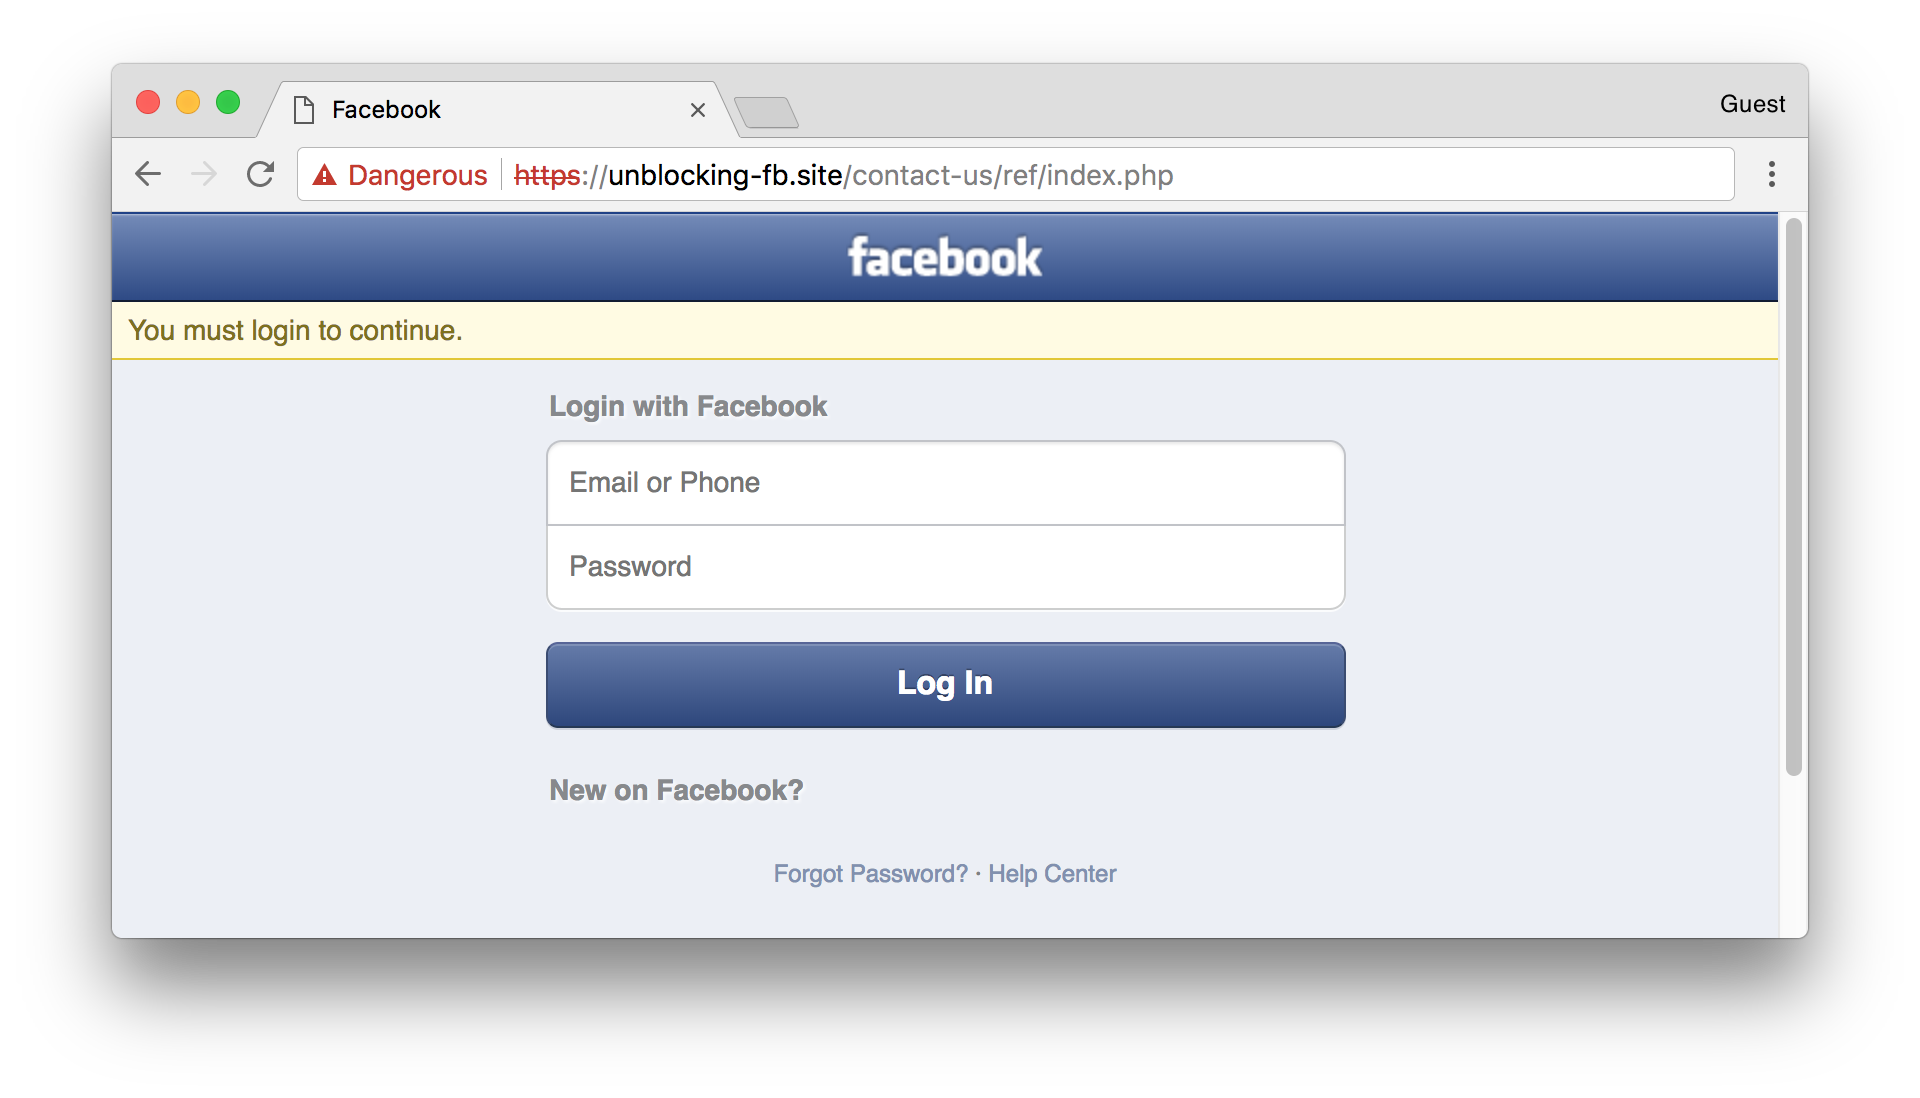
\includegraphics[width=0.7\linewidth]{rw/facebook-phishing-site}
	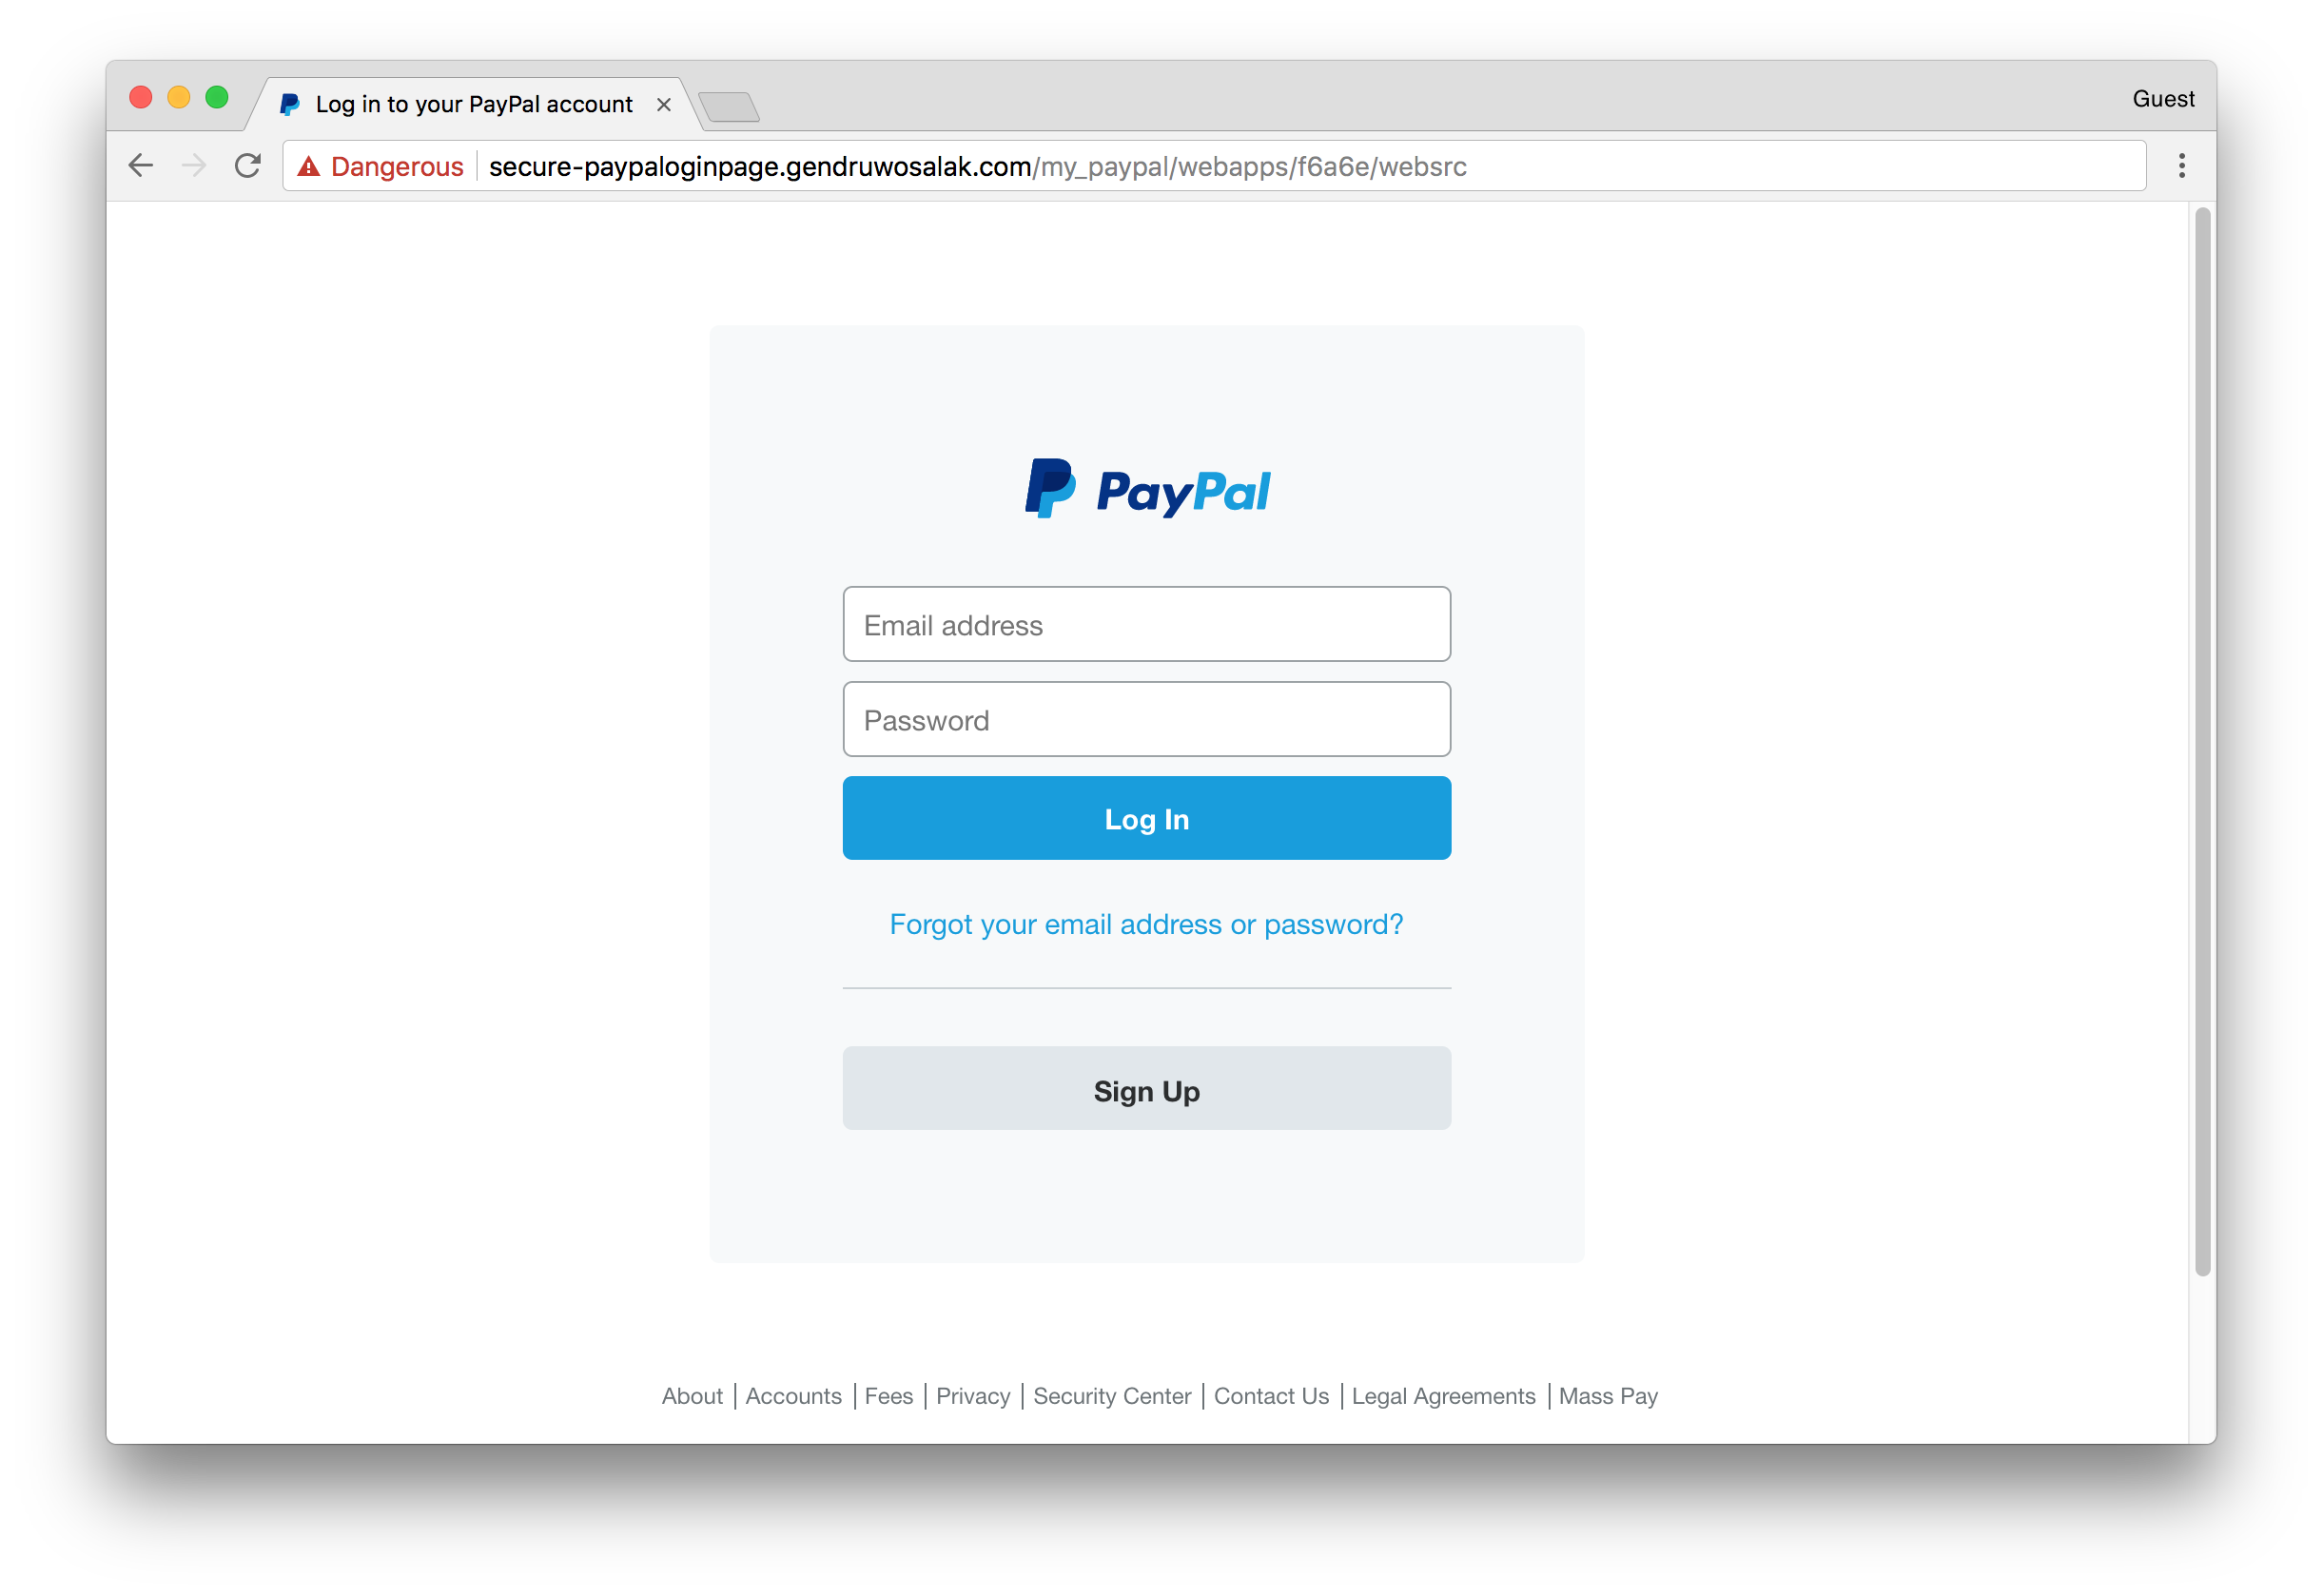
\includegraphics[width=0.7\linewidth]{rw/paypal-phishing-site}
	\caption{\label{fig:rw:phishingsite} Actual phishing websites targeting the facebook and paypal (online and accessible on 21.12.2017). The URLs contain ``fb'' (short for facebook) and keywords like ``secure'' ``paypal'' which contribute to falsely trusting the authenticity of the sites.\todo{split into two figures}}
\end{figure}

%%%%%%%%%%%%%%%%%%%%%%%%%%%%%%%%%%%%%%%%%
%%%%
%%%% p h i s h i n g
%%%%
%%%%%%%%%%%%%%%%%%%%%%%%%%%%%%%%%%%%%%%%%
\paragraph{Phishing / Social Engineering} 
% definition / high level description
Social engineering has become one of the biggest threats for a user's passwords with a growing number of incidents and fierce financial damage \cite{BKA2016Bundeslagebild}. Former criminal hacker Kevin D. Mitnick, who calls himself a social engineer, defines the term like this:
\begin{quotation}
	``Social Engineering uses influence and persuasion to deceive people
	by convincing them that the social engineer is someone he is not,
	or by manipulation. As a result, the social engineer is able to take
	advantage of people to obtain information with or without the use of
	technology.'' \cite[Frontmatter]{Mitnick2003ArtOfDeception}
\end{quotation}
Put simply, an attacker fools a victim into revealing certain kinds of information, including passwords. The most common social engineering attack on passwords is phishing, which typically involves two components: a fraudulent website that mimics another service and an email that lures the user onto this website \cite{Dhamija2006WhyPhishingWorks,Sheng2010WhoFallsForAPhish}. The email usually utilizes persuasive techniques like scaring  (``we noticed someone logged into your bank account and you need to reset your password'') time pressure (``you need to act \textit{now} to avoid further damage''). If the website looks just like the original (like the webpage in Figure \ref{fig:rw:phishingsite}), users might fall for it and enter their password to log in. In that case, it does not matter whether it is a strong, complex password or simply 12345 -- the attacker knows the username/password combination from that point on \cite{Tari2006ShoulderSurfingComparison}. If this tuple is used on other services, the attacker immediately gains access to them as well. 

% user perspective and mitigations
It is very challenging for users to validate the authenticity of a given webpage \cite{Dhamija2006WhyPhishingWorks, Fogg2001WhatMakesSitesCredible}. Usually, the URL is the best indicator, Dhamjia \etal among others argue that it is unrealistic to keep an eye on the URL at all times. Since the URL and padlock-icons are often ineffective, much research has been dedicated to help users in this validation and prevent phishing attacks. For example, Lin \etal found that domain highlighting in the URL bar only has a small effect on the effectiveness of phishing attacks, even after their participants were explicitly instructed to take not of the URL \cite{Lin2011DomainHighlighting}. Wu \etal showed that browser toolbars do not really help users, either \cite{Wu2006SecurityToolbars}. Dhamija \etal proposed a \textit{trusted path} between the user and the legitimate service \cite{Dhamija2005DynamicSecuritySkins}. In this system, users are supposed to verify the authenticity of a given website by comparing visual patterns in a trusted window and on the website. Together with Max-Emanuel Maurer and Alexander De Luca, I created a browser extension to visualize the usage of different types of SSL certificates across websites through the entire browser skin \cite{Maurer2011ShiningChrome}. We deployed it publicly and launched a feedback survey, which indicated that changing the browser skins is obtrusive enough to raise awareness and makes users more confident while browsing the Web. Until the recent change of platform APIs\footurl{https://blog.mozilla.org/addons/2017/11/20/extensions-in-firefox-58/}{21.12.2017} and resulting incompatibility problems, the extension named ``SSLPersonas'' had seen 47000 downloads, which is an indicator of both the necessity and the success of our solution. 

%% better solution: Browser prevents it by blocking phishing sites
However, optimally the browser would detect phishing websites and prevent that users visit them in the first place. Current versions of the major browsers try to do this and urge the user to leave the site, as is shown in Figure \ref{fig:rw:browser_warning}. This gives attackers only a short time-frame until the webpage has been classified as phishing, which takes 15 hours on average according to a recent Webroot report \cite{Girtakovskis2017WebrootThreatReport}. Older sources report a bit longer lifespans between 20 hours\footurl{https://www.lightbluetouchpaper.org/2007/05/16/how-quickly-are-phishing-websites-taken-down/}{21.12.2017} and 54 hours\footurl{https://news.netcraft.com/archives/2004/08/14/life_span_of_a_phishing_site_averages_54_hours.html}{21.12.2017}. 

%%%%
%%%% Browser Warning deceptive website.
\begin{figure}
	\centering
	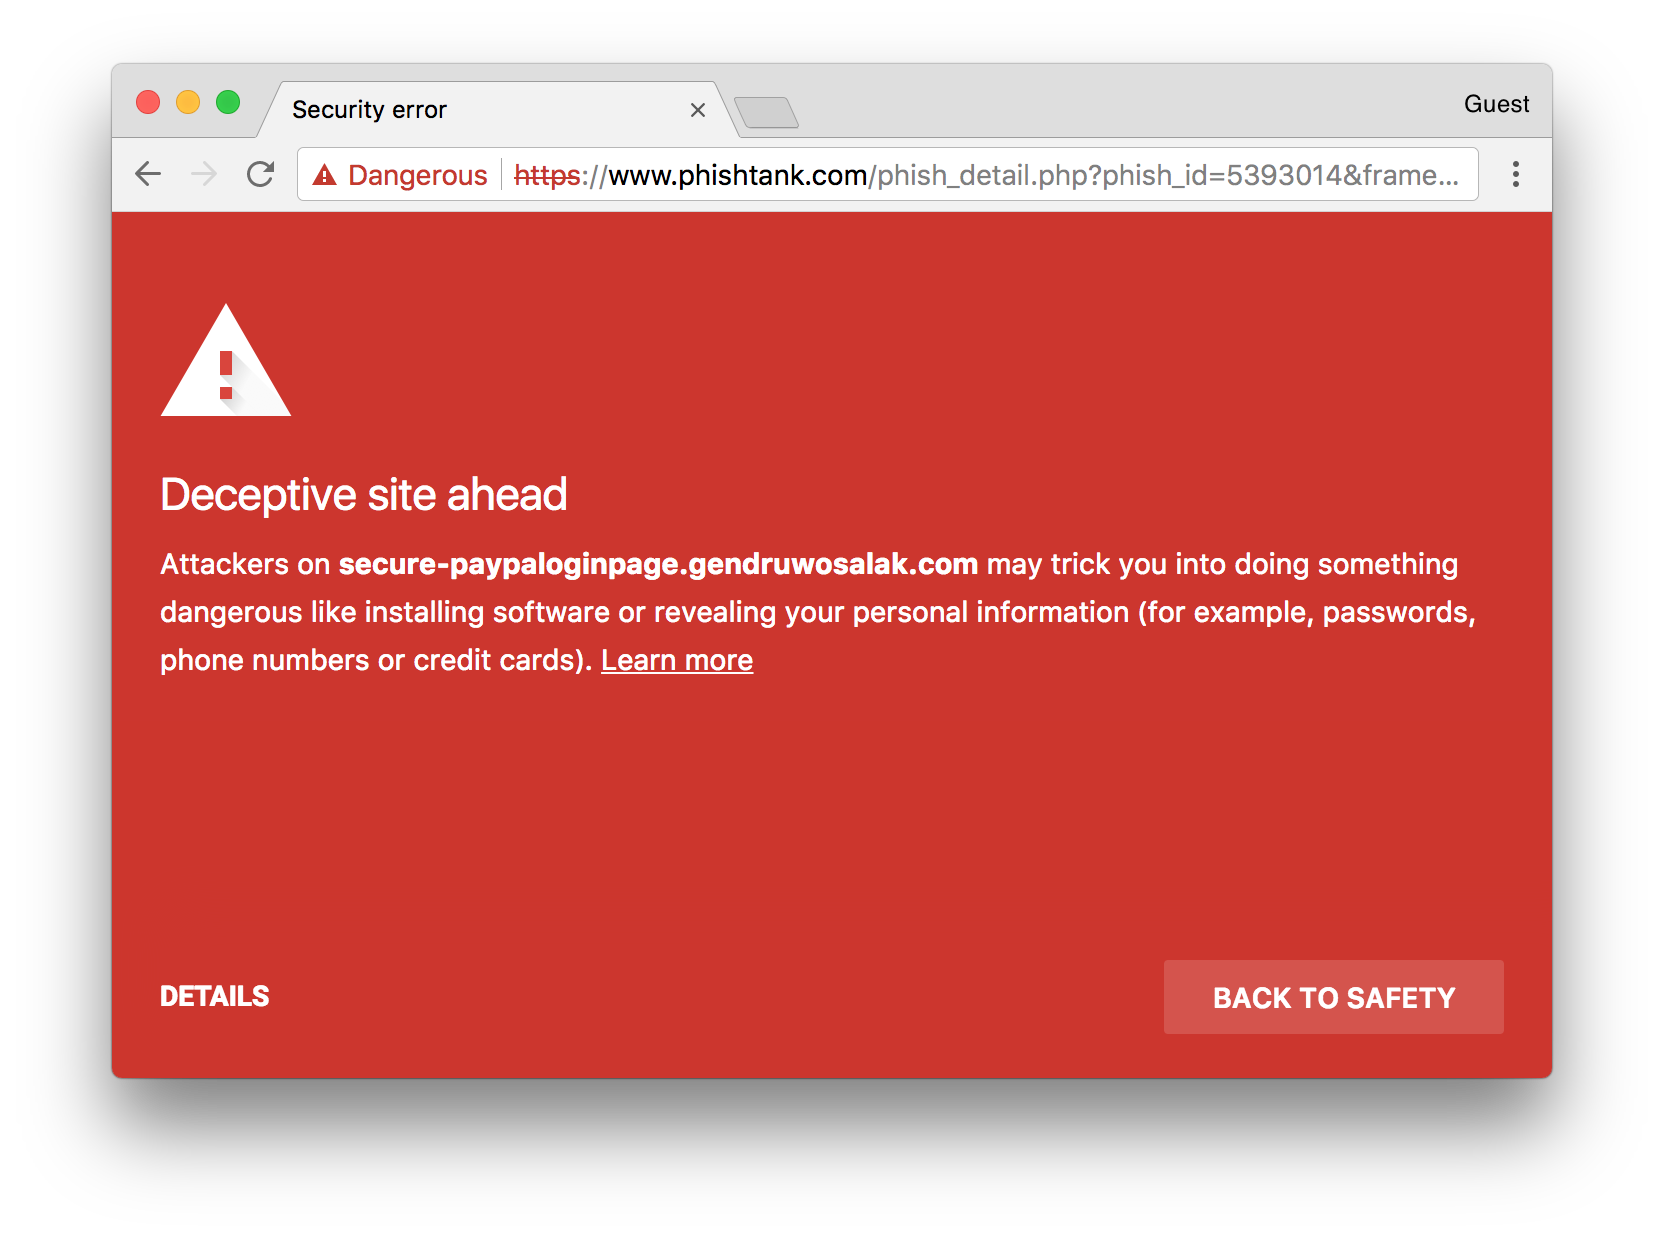
\includegraphics[width=0.8\linewidth]{rw/browser-warning-deceptive-site}
	\caption{\label{fig:rw:browser_warning}Chrome v63's warning on a phishing website. The user is urged to leave the site but still has the chance to visit it by clicking on ``Details''.}
\end{figure}

%%%%%%%%%%%%%%%%%%%%%%%%%%%%%%%%%%%%%%%%%
%%%%
%%%% m a l w a r e
%%%%
%%%%%%%%%%%%%%%%%%%%%%%%%%%%%%%%%%%%%%%%%
\paragraph{Malware and Eavesdropping} 
% attack description and types: keylogger.
Secretly stealing plain-text passwords is also possible by infiltrating the user's system with \textit{malware}, which is a term for \textit{mal}icious soft\textit{ware} \cite{Bayer2009CurrentMalware}. One of most common attacks is to install a keylogger that sends all keystrokes to the attacker. For the most part, this either happens as a ``drive-by-download'' when the user visits an infected website or by opening a malicious email attachment \cite{BKA2016Bundeslagebild}. In the former scenario, the sole line of defense lies with the service provider who needs to make sure their website is not infected.
% user perspective
Wash identified that users are aware of this kind of threat, but their mental model of malware is sub-par \cite{Wash2010FolkModels}. Hence, the countermeasures taken by the users are often insufficient. As with the phishing scenario, a strong password is incapable of preventing a malware attack. Ideally, users use an anti-virus solution, keep their software updated at all times and refrain from opening suspicious email attachments. 

% man in the middle attakcs
Moreover, user credentials can be intercepted in transit, e.g. after the user submits them through a web form. These so called man-in-the-middle attacks are tough to carry out, but strong passwords do not prevent them either. 
% solutions
One of the typical solutions to minimize the risk is encrypting the traffic with a secure protocol like SSL/TLS \cite[p. 853ff.]{Tanenbaum2011ComputerNetworks}, which is based on a public/private key infrastructure. This makes it harder for an adversary to act as the man in the middle, because they usually do not possess the necessary private key of either party. Attackers must tamper with the certificates which usually causes browsers show a warning \cite{Maurer2011ShiningChrome}. 
% user perspective 
Users, however, do not necessarily understand such warnings, because their understanding of the technical details is low \cite{Herley2009SoLongThanksExternalities, Whitten1999WhyJohnnyCantEncrypt}. Consequently, the HCI community has invested much effort to convey the essential messages in a clear and actionable way \cite{Felt2015ImprovingSSLWarnings, Felt2014ChromeSSL,  Maurer2011ShiningChrome, Sotirakopoulos2011ReplicationSSLWarnings, Sunshine2009CryingWolf}.

%Keyloggers, eavesdropped communication (e.g. via Man in the Middle Attacks)

%%%%%%%%%%%%%%%%%%%%%%%%%%%%%%%%%%%%%%%%%
%%%%
%%%% o b s e r v a t i o n 
%%%%
%%%%%%%%%%%%%%%%%%%%%%%%%%%%%%%%%%%%%%%%%
\paragraph{Observation} 
%what's the problem? how does the attack work? what are countermeasures from a technical side? what are countermeasures for the users? do strong passwords help? skill level required by the attacker?
To obtain the password of a specific user, one can also simply watch them enter it and figure out what the password was. This attack is typically referred to as ``shoulder surfing'' because the person who watches figuratively ``surfs'' on the user's ``shoulder'' to look at their screen \cite{Tari2006ShoulderSurfingComparison}. Shoulder surfing is relatively easy and does not require technical sophistication. But, although friends and family can carry out such an attack, it is safe to say that it is more problematic in public spaces where unknown bystanders are present. Typical interactions that take place in such environments can be found with PIN entry, e.g. on an ATM, or entering any kind of password on a mobile device, e.g. on a bus in close vicinity to other people. 
% new system as countermeasure: De Luca / ColorPIN
De Luca \etal dedicated some research to both scenarios. For instance, they investigated contextual factors during ATM usage and the design space for alternative ATM authentication mechanisms \cite{DeLuca2010UnderstandingATMSecurity}. They developed the ColorPIN scheme \cite{DeLuca2010ColorPIN}: Additionally to the number sequence, the user needs to memorize a \textit{color} sequence, e.g. 1 (\textbf{black}) - 2 (\textcolor{red}{\textbf{red}}) - 3 (\colorbox{black}{\textcolor{white}{\textbf{white}}}) - 4 (\textbf{black}).
Entering the PIN is done through indirect input: Instead of prompting the user to enter the digits directly on the keypad, the system displays digits accompanied by three distinct letters in black, red, and white underneath. The keyboard through which the ColorPIN is entered, shows each letter three times -- once in each color. To enter the ColorPIN, the user needs to first identify the correct digit (e.g. ``1''), and then type the corresponding letter in the right color (e.g. a black ``Q''). After each entered character, the letter assignment is randomized again. All of this makes it challenging for a shoulder surfer to quickly observe and learn the user's PIN by overwhelming their short-term memory \cite{Dunphy2010CloserLookGraphical}.

% it's mostly PINs and graphical passwords rather than alphanumeric ones
Moreover, long alphanumeric passwords are a seldom research topic with regard to shoulder surfing. Shaub \etal looked into the effect of different designs of virtual keyboards on shoulder surfing susceptibility \cite{Schaub2012PasswordShoulderSurfing}. Somewhat unsurprisingly, they found that keyboards with more cumbersome access to special characters are less prone to shoulder surfing because it is harder for an attacker to keep track of the keyboard switches. We can see in the ColorPIN example, PINs and graphical passwords are more likely to be under attack. Users usually enter graphical passwords more slowly \cite{Tari2006ShoulderSurfingComparison, Wiedenbeck2006ConvexHull, Renaud2009VisualSnakeOil}, which on the one hand gives an attacker more time to observe, but on the other hand burdens the short-term memory a bit more. Also, some visual authentication mechanisms require more screen real estate than a username/password form and entry is often not masked \cite{Biddle2009GraphicalFirstTwelveYears}. Still, there is not a lot of evidence that observation is a severe threat in the real world, other than for ATM PINs and any kind of credentials of people of public interest. Herley and Pieters point out that the attack is not scalable via algorithms like offline guessing \cite{Herley2015Counterfactuals}. Hence, Maguire and Renaud come to the conclusion that ``shoulder-surfing may well be a non-issue in authentication design'' \cite{Maguire2012YouOnlyLiveTwice}. 
% what about shoulder surfing on the web?
Using desktops or laptops to authenticate on regular websites, observation is rarely a major concern. Passwords are usually masked in the browser with an asterisk per character. However, this approach has recently been questioned because it prevents proactive error checking on the user side \cite{Sasse2016DebunkingMyths}. 

%%%%%%%%%%%%%%%%%%%%%%%%%%%%%%%%%%%%%%%%%
%%%%
%%%% o t h e r    a t t a c k s
%%%%
%%%%%%%%%%%%%%%%%%%%%%%%%%%%%%%%%%%%%%%%%
\paragraph{Other attacks} 
Apart from the attacks described above, there are other approaches that should not go unmentioned. First, people in one's own social circle, e.g. friends and family, have much personal information and often physical access to devices and passwords written onto post-it notes. Although the intent is often not purely malicious, it can be easy for these people to have an informed guess of a user's credentials. Flechais \etal use the term ``spouse attack'' to describe this kind of threat \cite{Flechais2013SaudiArabiaTrust}, Dunphy \etal call it a ``friend attack'', while Sasse and Flechais framed it as ``insider attack'' \cite{Sasse2005UsableSecurityPosition}. Ur \etal found that users underestimate its likelihood \cite{Ur2016PerceptionsPassword}. A strong, complex password that is only memorable to the legitimate user might help in that scenario. Weirich and Sasse, however, argue that such a strategy could make the user appear ``paranoid'' \cite{Weirich2001PrettyGoodPersuasion} and Flechais \etal see it as an important sign of trust \cite{Flechais2005DivideConquerTrust, Flechais2013SaudiArabiaTrust}. 
 
%%%% unintentional disclosure / discovery
Finally, some credentials are shared unintentionally on the web. Software developers who share open source code on the web are prone to this issue \cite{Conklin2004PWAuthenticationSystemPerspective}. Recently, the node package manager (npm) platform realized that many of its users published their passwords with the packages\footurl{http://blog.npmjs.org/post/161515829950/credentials-resets}{22.12.2017}. An adversary could simply crawl public repositories on GitHub and collect the passwords in plain text. The npmjs.org operators had to invalidate the credentials to secure the accounts. One solution that reduces the severity of credential loss is using multi-factor authentication (cf. Section \ref{sec:rw:shared_auth_tokens}).


%%%% 
%%%% TABLE: Attacks and Countermeasures
% Table generated by Excel2LaTeX from sheet 'attacks-mitigations'
\begin{table}[htbp]
  \centering
  \caption{\label{table:rw:attacks_countermeasures}Threats on passwords and potential countermeasures for users and service providers (SP). Other stakeholders are left out of this analysis.}
    \begin{tabular}{rll}
    \multicolumn{1}{l}{\textbf{Threat}} & \textbf{Countermeasures} & \textbf{Responsible} \\
    \hline
    \multicolumn{1}{l}{\textbf{Online Attack}} & Throttling & SP \\
          & Anomaly detection & SP \\
          & Set-up Multi-factor authentication & SP \\
          & Moderately complex password & User \\
          & Enable Multi-factor authentication & User \\
    \multicolumn{1}{l}{\textbf{Offline attack}} 
        	& Slow hash algorithm & SP \\
			& Secure database design & SP \\
			& Security audits, fix vulnerabilities & SP \\
		    & Complex, strong password & User \\

    \multicolumn{1}{l}{\textbf{Phishing}} & Education and Warnings & SP \\
    & Unique passwords & User \\
          & Check security indicators & User \\
          & Utilize spam filter & User \\
          & Vigilance regarding emails & User \\
    \multicolumn{1}{l}{\textbf{Malware}} & Anti-Virus software & User \\
          & Caution on the web & User \\
    \multicolumn{1}{l}{\textbf{Observation}} & Password masking & SP \\
    	& Awareness of surroundings & User \\
    \end{tabular}%
\end{table}%
%%%%
%%%%

%TODO Florêncio \etal proposed a classification for attacks \cite{Florencio2014PasswordPortfoliosFiniteUser}. Class 1-3

%OPTIONAL what is an attack ``vector''? attack steps from start to success. \ar
%Sometimes combinations of attacks (vector)

The main objective of this thesis is combating online and offline attacks, i.e. for algorithmic attacks, where password coping strategies really make a difference. A panacea for all kinds of threats, each of which has warranted multiple PhD theses, is probably impossible to find. 



%%%%%%%%%%%%%%%%%%%%%%%%%%%%%%%%%%%%%%%%%
%%%%
%%%% w h a t    i s    p a s s w o r d    s t r e n g t h
%%%%
%%%%%%%%%%%%%%%%%%%%%%%%%%%%%%%%%%%%%%%%%
\section{What is Password Strength? Metrics and Statistics}\label{sec:rw:pw_strength_metrics}
Bishop and Klein stated in 1995: ``A good password is one that is easily remembered, yet difficult to guess.'' \cite[p. 231]{Bishop1995ProactivePasswordChecking}. The second part of this statement describes password \textit{strength} on a high level. But there are problems if we try to objectively measure the ``difficulty to guess'' a password: is it difficult for an attacker with nearly unlimited resources, or only for an attacker that can only attempt once a day due to lock-out mechanisms? The question is highly context dependent and there is unfortunately no single true answer. 

Moreover, while ``\texttt{\{X@T;cuXw[bJnUH}'' is a randomly generated password that seems difficult to guess, it does not necessarily have to be a \textit{strong} password (see Section \ref{sec:rw:whats_a_bad_pw}): if it was found in a password database after a data breach, it is likely to be included among the first guesses in subsequent dictionary attacks. The number of leaked passwords has steadily increased in the past few years and thus has rendered many such strong passwords unsuitable (see footnote \ref{foot:rw:breachlevelindex}). In the same vein, Yang \etal state: ``If a strategy is widely used, then attackers may develop strategy-specific methods which can efficiently guess the passwords'' \cite{Yang2016MnemonicSentenceBased}. Economists call this the ``Tragedy of the Commons'' \cite{Hardin1968TragedyCommons}. This, for example, implies that if passphrases (cf. Section \ref{sec:rw:passphrases}) do become commonplace, attackers will optimize their attack strategy rendering the well-intended efforts to strengthen passwords less effective. Consequently, the challenge of considering such effects and realistically measuring password strength has sparked some discussion, which has led to a small set of suitable models which are discussed below.



	\subsection{Entropy}
	% information theoretical entropy
	In 1951, Claude Shannon put forward an information-theoretical approach that describes the encoding of English letters and words \cite{Shannon1951Entropy}. In there, he defines the term ``entropy'' as ``\textit{a statistical parameter, which measures [...] how much information is produced on the average for each letter of text in the language. If the language is translated into binary digits (0 or 1) in the most efficient way, the entropy H is the average number of binary digits required per letter of the original language}''. In other words, entropy represents the amount of information of a given word in bits. 
	
	% high level entropy description as understood by NIST
	William (Bill) Burr and his colleagues at \gls{NIST} took to this understanding and translated it into a measure for password strength, which was officially published for the first time in 2004 \cite[Appendix A]{Burr2004NISTEntropy}. They define ``guessing-entropy'' as ``an estimate of the average amount of work required to guess the password of a selected user''. Apart from guessing a single user's password, the macro perspective defines the ``min-entropy'' as ``a measure of the difficulty of guessing the easiest single password to guess in the population''. Although many citing publications (e.g. \cite{Egelman2013DoesMyPasswordGoUpToEleven,Bonneau2012ScienceOfGuessing}) do not sufficiently point it out, Burr \etal explicitly acknowledge the limitation of using entropy as metric for user-selected passwords. They base their estimate on frequency distributions, meaning more frequently used passwords are guessed first and are thus lower in entropy. 
	
	% random passwords.
	For random passwords, the \gls{NIST} guideline gives the following entropy calculation formula. 
	
	$$ H = log_2(b^l)$$
	
	\textit{b} is the size of the alphabet, e.g. the 94 ISO-printable characters, and \textit{l} is the length of the password. For an 8-character password this would give an entropy of $log_2(94^8)~=~52~bits$. 
	
	% that won't work for user selected passwords and NIST already knows it.
	Most users do not use random passwords (for a detailed discussion see Section \ref{sec:rw:user-behavior}), therefore this kind of entropy calculation is rarely realistic. In other words, the effective or practical password space is much smaller than the theoretical password space. The \gls{NIST} guideline tries to take this into account and gives another calculation approach based on user behavior (see page 49f. in \cite{Burr2004NISTEntropy}). It lists a few entropy heuristics, e.g. the first character gives 4 bits of entropy, the next 7 characters add 2 bits of entropy each, while the 9th through 20th character only add 1.5 bits. Burr \etal do not provide a formal rationale as to why this was chosen. But again, the publication specifically points out that this is still an inaccurate approach because this would require ``examining in detail the passwords that users actually select under the rules of the password system''. Moreover, they admitted that ``NIST would like to obtain more data on the passwords users actually choose, but, where	they have the data, system administrators are understandably reluctant to reveal password	data to others''. In the meantime, however, there have been many data leaks which fill this hole (see Table \ref{tab:rw:password_leaks}).
	
	\subsection{Guess Numbers: Markov Models, PCFGs, and Neural Networks}
	
	% Weir algorithm: PCFG
	Using such leaked data, Weir \etal developed a probabilistic context free grammar (PCFG) cracking method in 2009 \cite{Weir2009PCFG}. The idea behind PCFG is that passwords often follow a rather predictable scheme (e.g. a word followed by a sequence of digits and an exclamation mark, see Section \ref{sec:rw:user-behavior}). One can model such patterns with so-called mangling rules. Weir \etal's approach was to find a set of mangling rules that crack the most passwords in a given data set. A mangling rule takes a certain password input and creates one or more alternative versions of it, for instance the rule could be to replace all occurrences of the letter ``s'' with the ``\$'' symbol (password would become pa\$\$word). The ultimate goal is to minimize the number of guesses to crack passwords. Mangling rules also are essential for password cracking software like John the Ripper or Hashcat, but those tools primarily use them to generate word-lists, and not for guessing-order optimization. Veras \etal \cite{Veras2014SemanticPatterns}, as well as Komanduri extended Weir \etal's PCFG approach afterwards \cite{Komanduri2016Dissertation}.

	% Weir against NIST
	A year later, Weir \etal evaluated the usage of the \gls{NIST} entropy formulae against real-world passwords and policies \cite{Weir2010MetricsPolicies} to address the issues pointed out by Burr \etal. For the evaluation, they performed guessing attacks with PCFG on leaked password sets (most notably RockYou). As a comparison they calculated the NIST entropy for each password and correlated it with cracking success rates. Their analyses show that the calculated entropies were not satisfyingly predictive of cracking success, and they concluded that \textit{``there is no way to convert the notion of Shannon entropy into the guessing entropy of password creation
	policies''}. Weir \etal thus proposed ``guessing probability'' as a more accurate password strength metric and the result of an analysis is a kind of lookup-table split into different probability groups. 

	% Kelley agorithm
	Since the computing power required to perform the PCFG attack was relatively high, Kelley \etal tried to improve the algorithm by testing multiple training sets and variations of guess algorithms \cite{Kelley2012GuessAgain}. They used the Mechanical Turk platform to collect new passwords created under different policies (more on policies in Section \ref{sec:rw:policies}) and tried to crack them. Tuning the right parameters for cracking by exploiting a priori knowledge (e.g. password policy) led to much more cost-efficient analyses, but the training still takes approximately 24 hours. However, once the Markov-chain model is generated, one can simply pass in any kind of password and retrieve its \textit{guess number}. The higher the guess number, the stronger it is. After a certain threshold, the password is considered unguessable -- which is also one of the limitations of the approach. Kelley \etal's approach soon became a gold standard to measure password strength, especially at CMU. Komanduri \etal were probably the last ones in 2011 that still used entropy as strength metric \cite{Komanduri2011OfPasswordsAndPeople}. Kelley \etal's guess numbers caught on and are still used today, perhaps because they directly represents the \textit{``number of attempts that an attacker would need in order to guess it''} \cite{Dellamico2015MonteCarlo} or as Carnavalet put it \textit{``the amount of effort an adversary must employ to break the password''} \cite{Carnavalet2014AnalyzingPWStrengthMeters}.
	
	% Bonneau
	Almost simultaneously to Kelley \etal, Bonneau developed his idea of efficient and effective guessing, which has also generated a lot of impact since then \cite{Bonneau2012ScienceOfGuessing}. He collected leaked passwords and tried to attack them in different ways to find patterns in user behavior that could be leveraged in real-world attacks. Fundamentally, the attacks different in the choice of dictionaries. He found that the success rates strongly depend on the dictionary that is used for it. He aimed to translate his findings to a new entropy paradigm and concluded that 10 bits of entropy are probably enough to defend against online attacks, respectively 20 bits for offline attacks. 
	
	% Ur guessing / PGS	
	Ur \etal took guessing to the next level by evaluating the most sophisticated approaches to date against each other \cite{Ur2015MeasuringRealWorldAccuracies}. They compared the performance of John the Ripper, Hashcat/oclHashcat, Markov chains/PCFG and professional password recovery companies. Moreover, they tested several configurations of the tools and checked their guess success rates for passwords created under different password policies. They conclude that a multi-tiered approach is capable of giving the most conservative metric password strength. One of their major contributions of this work is the Password Guessability Service (PGS) that they since offer\footurl{https://pgs.ece.cmu.edu/}{27.12.2017}. After successful registration, researchers can upload a file containing plain-text passwords, e.g. after collecting them through a user study (cf. Section \ref{sec:rw:methodology}). The user has to provide a few additional parameters, like the policy that was utilized, which enhances the guessing efficiency and reliability. Then a set of cracking approaches are run in parallel and the analysis is sent back to the uploader. 
	% PGS limitations (oops this looks a lot...)
	Although this has become an established, state-of-the art tool which has already been used in numerous publications (e.g., \cite{Gross2016CognitiveDepletion, Habib2017Blacklists, Mcevoy2016ContextualizingMnemonicPhrase, Segreti2017AdaptivePolicies, Ur2017DataDrivenPWMeter, Wheeler2016zxcvbn}), it does not come without caveats. First, passwords need to be uploaded in plain text. This entails a more careful handling and storage if they originate from a user study, because users might in fact have used their real-world passwords (see \ref{sec:rw:methodology}). Plain-text passwords also imply that users disclosed them somehow and the mere act of disclosing might already reduce the strength of passwords, which is not factored into the guess numbers. However, the team at CMU counteracts this problem by deleting uploads after at most two weeks. Besides, the analyses are time-consuming, and obtaining results can in fact take several weeks, because the system is shared with other users. Moreover, if a study aims to compare multiple password policies, each condition needs to be separately uploaded and subsequently analyzed. Finally, in personal conversations with the research team, they pointed out that certain unicode characters are not supported. This makes it infeasible for passwords that were collected in countries whose languages heavily use umlauts (ä,ö,ü). Nevertheless, it appears to be one of the best strength proxies the community has at the moment. 

	% finally: neural networks.	
	A rather novel approach that has not been integrated into the PGS are cracking algorithms based on neural networks. Melicher \etal demonstrated an opportunity to configure such algorithms to  perform better than former state-of-the-art techniques like PCFG and Markov models \cite{Melicher2016NeuralNetworks}. They implemented neural networks based on Monte-Carlo simulations, i.e. ``smart sampling'' (cf. \cite{Dellamico2015MonteCarlo}). A thorough evaluation against PCFG, Markov-models, and word-list crackers showed that neural networks can outperform all of them if properly trained. Moreover, Melicher \etal were also able to implement their approach in JavaScript. This highlights one major advantage of using neural networks: once the model has been trained, it can be packaged and shipped to browsers, which only requires a few hundred kilobytes. They showed that this type of client-side strength estimation fares really well. One caveat is that the solution does not work ``out of the box''. Developers have to train their models and this means that faulty configurations might lead to erroneous strength estimations. 
	
	\subsection{The zxcvbn Approach: Lightweight, Robust, Simple}\label{sec:rw:zxcbn}
	Daniel Wheeler presented an approach towards password strength estimation by providing a conservative expected guess-number \cite{Wheeler2016zxcvbn}. We take a closer look at it, because it served as a strength metric for much of the work in this thesis. 

	% how zxcvbn works.
	Similar to PCFG and mangling rules, the idea is based on pattern matching against dictionaries and leaked password corpora. The result is a calculation of the minimum rank over a series of frequency ranked lists, i.e. a guess number. In other words, the approach is \textit{heuristic} instead of \textit{probabilistic}, because the rank is based on \textit{searching} through the patterns. The pattern-ranks themselves are not necessarily based on likelihoods, but on a search sequence that may lead to different prioritization of heuristics depending on the found patterns. The implementation of the algorithm is called zxcvbn\footnote{The name zxcvbn originates from the bottom row on a QWERTY keyboard. Many users mistakenly consider this approach secure because the resulting password looks fairly random.}. Wheeler showed that in an online attack scenario \cite{Florencio2014AdministratorsGuide} the algorithm estimates the number of guesses accurately within an order of magnitude of 2 -- consistently better than \gls{NIST} guidelines to date and other lightweight strength estimators. Beyond the online-attack threshold, the results are mixed, but adding more tokens to the dictionary further improves robustness. Moreover, zxcvbn provides a numerical password score from 0 to 4. The README describes the thresholds, which are motivated through different attack scenarios (see Section \ref{sec:rw:attack_vectors}):
	
	\begin{description}
		\item[0] too guessable: risky password -- guess number < $10^3$
		\item[1] very guessable: protection from throttled online attacks -- guess number < $10^6$
		\item[2] somewhat guessable: protection from \textbf{un}throttled online attacks -- guess number < $10^8$
		\item[3] safely unguessable: moderate protection from offline slow-hash scenario -- guess number < $10^{10}$
		\item[4] very unguessable: strong protection from offline slow-hash scenario -- guess number $>=10^{10}$
	\end{description} 

	These steps are plausible and can be derived from academic literature, e.g. \cite{Bonneau2012ScienceOfGuessing, Florencio2014AdministratorsGuide, Ur2015MeasuringRealWorldAccuracies, Wang2016fuzzyPWM}
	
	% benefits
	One of the advantages of zxcvbn is that its implementation is fairly small (1.5 Megabytes in total). It comes with 100,000 tokens which allows zxcvbn to conservatively estimate the guess numbers. Moreover, it can be extended with site-specific word-lists. Zxcvbn performs its calculations within milliseconds, which makes it suitable to run strength analyses on the client. This is a major advantage, e.g., to provide users with real-time feedback on password strength. Moreover, it can also be easily used on the server to enforce more advanced password policies, e.g. with NodeJS. Since zxcvbn is open-source, one can modify and adapt it to meet context-dependent requirements. This makes it extremely useful for user studies: One can strip sensitive information from the analysis and save zxcvbn's output straight to a database, which is ethically reasonable and speeds up further analyses. 

	%limitations
	Despite the benefits, one needs to be aware of zxcvbn's drawbacks. Carnavalet compared several real-world password strength estimators, one of which was zxcvbn v2.x \cite{DeCarnedeCarnavalet2015PasswordMeters}. Although they concluded that zxcvbn was the best of the tested estimators, they see the major limitation in the static dictionary size. Zxcvbn ships with index terms from the English Wikipedia, English words from TV and movie subtitles, a list of roughly 47000 frequency-ranked passwords, female and male prenames, and surnames from English-speaking countries. Hence, all words that cannot be matched from these wordlists including mangling rules, are seen as random strings. Zxcvbn goes on to assume these can only be cracked by brute force, but real-world attackers possessing a priori knowledge of the target population might find ways to guess these passwords more efficiently. However, Melicher \etal's neural network suffers from similar limitations. For instance, Carnavalet and Mannan's \cite{Carnavalet2014AnalyzingPWStrengthMeters} example ``dolce\&gabana'' (an Italian luxury brand) receives a guess number 358000010000 $\approx 1e11.5$ from zxcvbn, and 2587762225797 $\approx 1e12.4$ from Melicher \etal's tool -- so both estimates are perhaps too optimistic. Finally, Carnavalet also critized that zxcvbn did not detect reversed words, but this heuristic was later added in version 3.5.0\footurl{https://github.com/dropbox/zxcvbn/releases/tag/3.5.0}{28.12.2017}. So although neural networks are a viable alternative, zxcvbn is one of the best estimators currently available. 
	
	% Impact on industry and research
	Zxcvbn's usefulness is underlined by its impact during the first years of its existence. In the industry, zxcvbn has become the standard password-checker on WordPress since version 3.7 \cite{DeCarnedeCarnavalet2015PasswordMeters}, and for Dropbox (zxcvbn's author works there). In academic literature it has received praise from Ur \etal \cite{Ur2017DataDrivenPWMeter}, Komanduri \etal \cite{Komanduri2014Telepathwords}, and Wang \etal \cite{Wang2016fuzzyPWM}. It was also actively utilized as strength proxy in by Groß \etal to measure associations between cognitive depletion and password strength \cite{Gross2016CognitiveDepletion}, by Yang \etal to study mnemonic phrase based passwords \cite{Yang2016MnemonicSentenceBased}, by Lyastani \etal to study the impact of password managers on password strength \cite{Lyastani2017ImpactPWMPasswordStrength} and also recently by Al-Jaffan to build a new strength visualization \cite{Aljaffan2017PasswordSecurityVisualizer}.
	
	All this made us confident to utilize zxcvbn in our own studies which are reported in later sections. 
	
	\subsection{Other strength proxies}
	Apart from entropy and guess numbers, not many strength metrics succeeded to become prevalent. For the sake of completeness, we briefly point out more related work on the topic. Most notably, Bonneau combined two \textit{partial guessing} metrics to go beyond entropy and guess work \cite{Bonneau2012ScienceOfGuessing}: From the $\beta$-success rate \cite{Boztas1999Entropies} and the $\alpha$-work-factor \cite{Pliam2000IncomparabilityEntropyGuesswork}, he derived the $\alpha$-guesswork metric. The former roughly describes the success rate of an attacker that is limited to $\beta$ guesses, while the $\alpha$-work factor denotes the mimimum required guesses to crack a desired proportion of $\alpha$ passwords. Yang \etal chose to solely rely on $\beta$-success rates \cite{Yang2016MnemonicSentenceBased}, although Bonneau discourages this in his PhD thesis \cite{Bonneau2012Thesis}. 
	
	Beside those metrics, Dell'Amico \etal investigated using a multi-level cracking approach to find a cut-off threshold (as strength metric) when an attack becomes infeasible \cite{DellAmico2010PasswordStrength}. In another paper, they use probabilities of succeeding with different cracking methods \cite{Dellamico2015MonteCarlo}. Finally, Li \etal incorporated personal information into PCFG and suggest a new metric named ``Coverage'' \cite{Li2017PersonalInformation}. Essentially, this proxy tells us how likely it is to crack a password if we obtain personal information of the user.
	
	In a sense, these additional strength metrics could be subsumed under ``guesswork proxies'', too. Until now, they have not seen significant attention in the community nor by the industry. Perhaps their success is a bit hampered because they do not provide a straight-forward interpretable calculation, respectively result, which makes other solutions like PGS, Neural Networks, and zxcvbn more attractive to researchers in HCI.
	

\section{What is a ``Bad'' Password?}\label{sec:rw:whats_a_bad_pw}
Having looked at strength metrics, it is fair to ask what exactly a ``bad'' password is. Unfortunately, the question is more or less impossible to answer, especially without context. The word ``bad'' is judgmental on its own and depends on whom is asked. A security expert might call a password ``bad'' if it only contains lowercase letters because she knows how to crack such passwords, but a regular mainstream user might call it ``bad'' because he cannot type it quickly enough or keeps forgetting it. So, it ``bad'' depends on one's own standards, knowledge, beliefs, preferences, and usage context \cite{Gaw2005ReuseRecycle, Haque2014Hierarchy}. There is a fine difference between the adjective pairs ``good''-''bad'' and ``strong''-``weak''. A weak password might still be \textit{good}, when it fits the purpose, i.e. when it is good \textit{enough}. For example, four-digit PINs are widely used to authenticate at ATMs. Theoretically, there are only 10000 possible combinations, which could be brute-forced within milliseconds. Still, the second factor (banking card) and lock-down mechanisms after a number of guesses effectively prevent such attacks, so PINs are \textit{good enough} for the purpose. As another example, a user might choose a dictionary word like ``\texttt{spacetime}'' to sign up for an online forum. If they do not reuse this password for a more important service like accessing emails, the seemingly weak password might still be \textit{good enough} for this purpose. Zhang-Kennedy \etal \cite{ZhangKennedy2016RevisitingPasswordRules} as well as Florêncio \etal \cite{Florencio2007DoStrongWebPasswords, Florencio2014AdministratorsGuide, Florencio2014PasswordPortfoliosFiniteUser, Florencio2016CommACM} seem to agree, and Herley and van Oorshot frame it nicely in \cite{Herley2012PersistenceOfPasswords}:

\begin{quote}
	``Fifth, when are offline attacks a threat? While dependent on implementation, access to salted hashed passwords requires attacker effort; long gone are the days when password hash files were by default world readable. A disgruntled ex-sysadmin who steals hashed passwords is the often-conjectured foe in this attack; yet, if untrusted individuals have had unfettered unaudited access to the authentication server, a site’s problems go well beyond password strength. Sixth, are there ways to protect against off-line attacks besides password strength? Mandating password changes once hashes leak might be better than strong policies at all times. Only if a leak goes unnoticed (and a password change isn't forced) does strength potentially help. Of course, reliably detecting leaks or break-ins itself remains difficult. Finally, how much strength is required to protect against offline attacks? The bar is clearly much higher than for online attacks (assuming lockout or rate-limiting policies in place), but at what strength are attacks effectively addressed?'' 
\end{quote}

So, in that vein, if we invert Bishop and Klein's definition, we would get ``A bad password is one that is hard to remember, yet easy to guess'' \cite{Bishop1995ProactivePasswordChecking}. Human capabilities must not be neglected, which is why we discuss it in detail in Chapter \ref{chap:rw:user_perspective}. But neither humans nor contexts are all equal, so the answer as to what a ``bad'' password is, remains a solid ``it depends''. Still, users sometimes seek for guidance (cf Section \ref{sec:rw:advice_guidance}) and continue to ask this question. Let us thus have a look at more practical answer rather than ``it depends''. Burnett provides a list of high-level heuristics that a user can decide to employ to figure out if their preferred password choice is ``bad'' \cite{Burnett2005PerfectPasswords} (excerpt, but directly quoted):
\begin{enumerate}
	\item If you typed your password in Google, would you get no results?
	\item Are you the only person who knows the password?
	\item If you have your password recorded somewhere, is it in a secure location?
	\item Do you remember your password without having to look it up?
	\item Can you type your password quickly without making mistakes?
\end{enumerate}
Bullets 1. - 3. are solely focused on security, while the remaining two are user-centered. He provides more heuristics, however, they are questionnable because they are demanding on the user's cognitive abilities. From related work, we can also derive more questions that generally aim at identifying inadequate passwords:
\begin{enumerate}\setcounter{enumi}{5}
	\item Is your password used by somebody else? \cite{Bonneau2012ScienceOfGuessing}
	\item Is your password short, that is, less than eight characters? \cite{Weir2010MetricsPolicies}
	\item Has your password leaked (check via \url{https://haveibeenpwned.com/})? \cite{Wheeler2016zxcvbn}
	\item Does your password only consist of personal information that can be found on your public social network profiles? \cite{Li2017PersonalInformation}
	\item \todo{FEEDBACK: if reviewers think the list is useful and should be extended, summarize more of these points}
\end{enumerate}

On a more opinionated level, I personally argue that a ``bad'' password is one that you \textit{care about}, but do not sufficiently try to protect against attackers in any scenario, although you are aware of better options. 

\section{Authentication beyond Passwords}\label{sec:rw:authentication_without_pws}
The benefits and drawbacks of using passwords have been studied extensively. Some drawbacks already become apparent when we recall Ali Baba's story: Ali Baba overhears the thieves saying the magic words and can immediately authenticate with them (a big security issue). He also told the ``password'' to his brother, but he fails to recall it (the biggest usability issue).

Table \ref{table:rw:benefits_drawbacks_pws} shows a high-level summary of the benefits and drawbacks that come along with password-based authentication. We can observe that the drawbacks constitute important constraints and it is natural to try to remove such limitations by considering alternatives. To give the reader a sense of the alternatives, this section briefly covers the most notable approaches to authenticate users without alphanumerical passwords or with additional security measures. 

	\subsection{Graphical Passwords \& Visual Authentication Methods}\label{sec:rw:graphical_pws}
	In 1995, Blonder filed a patent with the name ``Graphical Password'' \cite{Blonder1996PatentGraphicalPW}, which marked the beginning of a range of new authentication schemes: Graphical (or visual) authentication. The patent presented a mechanism that prompts the user to prove their identity through correctly clicking a number of locations in an image. His goal was to find an alternative to text-based passwords that is easier to remember, without losing security benefits \cite{Biddle2009GraphicalFirstTwelveYears, Renaud2009VisualSnakeOil}. Psychological studies have revealed that pictures are easier to remember than words, which is often referred to as the \textit{picture superiority effect} \cite{Paivio1968PicturesEasierThanWords}. Grady \etal state that it works the best if there is an episode that serves as mnemonic device \cite{Grady1998NeuralCorrelates}. A number of studies in HCI demonstrate the benefits of graphical authentication. For instance, Chiasson \etal report on a lab study which showed that graphical passwords are easier to remember and less error-prone in the short term \cite{Chiasson2009InterferencesGraphical}. In the long term, however, there was not significant difference to textual passwords. Elizabeth Stobert, who dedicated a large part of her PhD work to graphical passwords \cite{Stobert2015Dissertation}, also found memorability benefits \cite{Stobert2013GraphicalPasswords}. Beside, memorability benefits, there are other advantages like personalization and tailoring schemes to specific user groups. Imran found that graphical passwords are easily understood by children \cite{Imran2015PWsAdultsChildren}, while Carter presented a new effective system specifically designed for older adults \cite{Carter2015GraphicalPasswordsOlderUsers}. 
	
	In the 20 years that followed the patent grant, three different approaches prevailed: searchmetric, locimetric, and drawmetric systems. In the following we describe them and provide a few notable examples. 
		
	\paragraph{Searchmetric Systems}
	The idea behind all searchmetric (also recognition-based) systems is to recognize objects or images in a ``challenge set'' \cite{VonZezschwitz2016Thesis}, i.e., to \textit{search} for the correct image. The commercial PassFaces\footurl{http://www.realuser.com/}{29.12.2017} system is a paragon in this domain (see Figure \ref{fig:rw:searchmetric}). The user is challenged with identifying the picture of a person in a grid of nine pictures of people. To increase security, this challenge is executed three times in a row\footnote{The current implementation challenges the user three times, while the original proposal included four challenges.}. The three images the user needs to identify were chosen beforehand in the \textit{enrollment} stage. Brostoff and Sasse, found in a field study that users were able to log in with Passfaces even after a long period of inactivity \cite{Brostoff2000PassfacesEvaluation}. However, they also report that participants spoke unfavorably of Passfaces, because of the increased authentication time. By random guessing, an attacker would have a chance of $\frac{1}{9}*\frac{1}{9}*\frac{1}{9}~=~0.001$, \ie one in one thousand to find a user's faces. Davis \etal, however, found that user selection of Passfaces is predictable, thus reducing the effective password space \cite{Davis2004UserChoiceGraphical}. Dunphy \etal created a mechanism that is based on photos \cite{Dunphy2010CloserLookGraphical}. In a two-week field trial they found that participants successfully authenticated in 77\% of attempts, and human attackers needed between 4.5 and 7.5 observations to shoulder-surf the passwords. 
	
	Dhamija and Perrig created a similar mechanism called ``Déjà Vu'' \cite{Dhamija2000DejaVu}, where the user selects a number of random-art images instead of faces (see Figure \ref{fig:rw:searchmetric} B). Although participants in a lab study generally liked Déjà Vu, the system was never adopted on larger scope. Another alternative solution to using faces is VIP, which is based on pictures of objects \cite{DeAngeli2002VIP, DeAngeli2005PictureThousandWords}. They iteratively improved the prototype, and found that recognizing six simple and concrete objects worked the best, but was still much slower than entering a PIN. Bicakci \etal also explored authenticating through clicking a sequence of icons as master password for a password manager \cite{Bicakci2011PWMIconBased}. They found that some icons were more attractive than others and thus impaired security. An icon-based mechanism that strongly focuses on mitigating shoulder-surfing is Wiedenbeck \etal's Convex-Hull-Click (CHC) system \cite{Wiedenbeck2006ConvexHull}. The challenge set consists of icons which are randomly distributed in the grid. The idea behind CHC is that the user does not click on their enrolled icons, but anywhere inside the convex-hull which is formed by the icons. In other words, the user clicks a random icon within the virtual polygon that is formed by the icons if they were connected by straight lines. Wiedenbeck \etal showed that CHC has security benefits, but the large grid of icons negatively impacted authentication times. Moreover, Golla \etal, respectively Kraus \etal recently evaluated emojis instead of PINs for mobile phones \cite{Golla2017EmojiAuth, Kraus2017Emoji}. Contrary to traditional pins, the emojis are randomly ordered in the grid, which makes their system a typical ``searchmetric'' approach. The idea actually originates from ``Emoji passcode'', a commercial solution from Intelligent Environments but had never been formally evaluated until their studies \footurl{https://www.intelligentenvironments.com/now-you-can-log-into-your-bank-using-emoji/}{29.12.2017}. 
	
	% IMAGES - SEARCHMETRIC
	\todo{split figure and reference to individual images in text.}
	\begin{figure}[htbp]
		\centering
		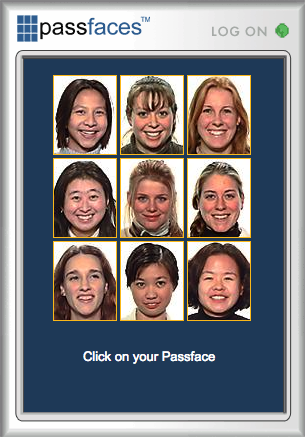
\includegraphics[width=0.3\linewidth]{rw/passfaces}
		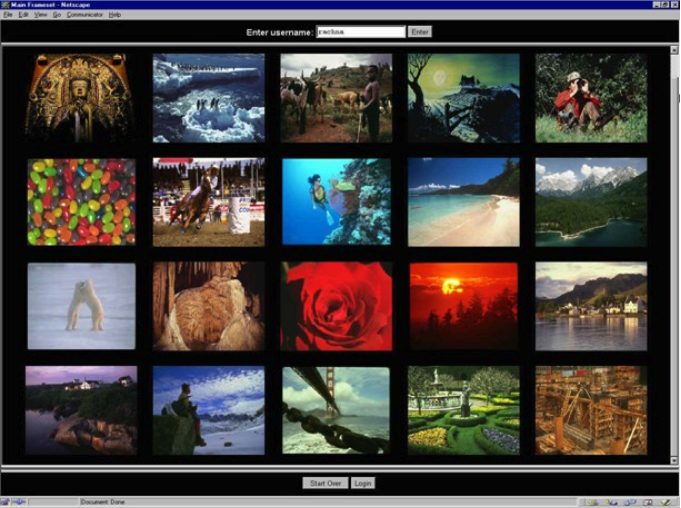
\includegraphics[width=0.55\linewidth]{rw/deja-vu-login-screen}
		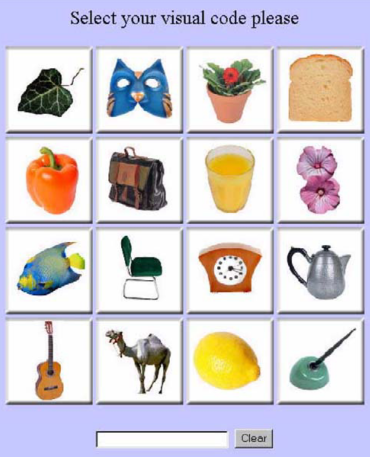
\includegraphics[width=0.3\linewidth]{rw/VIP-3-final}
		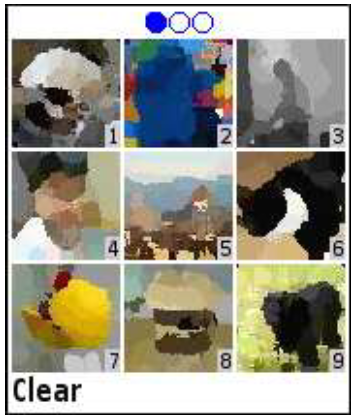
\includegraphics[width=0.3\linewidth]{rw/use-your-illusion}
		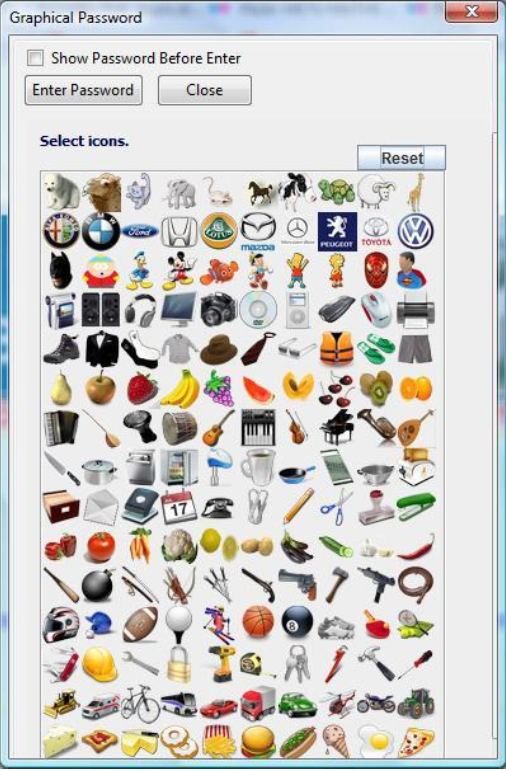
\includegraphics[width=0.3\linewidth]{rw/iPMAN}
		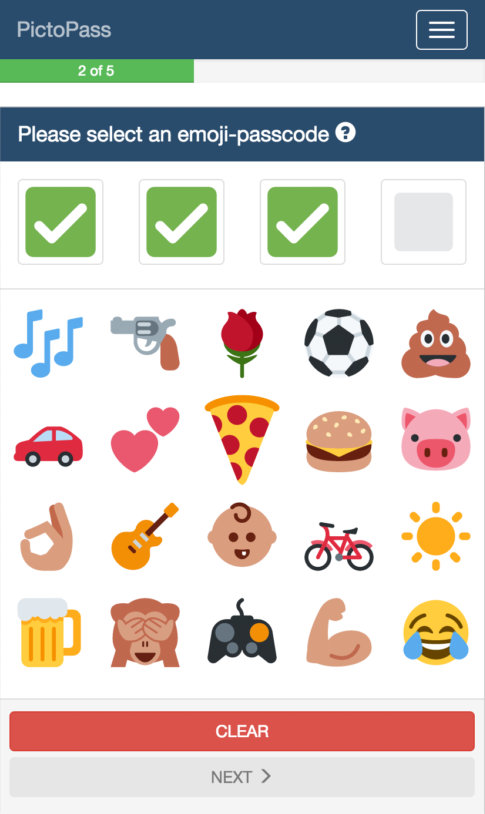
\includegraphics[width=0.3\linewidth]{rw/emojiauth}
		\caption{\label{fig:rw:searchmetric} A) PassFaces B) Déjà Vu C) VIP 3, final prototype D) Use Your Illusion E) iPMAN F) EmojiAuth / Pictopass}
	\end{figure}
	
	Hayashi \etal went beyond image recognition and blurred images during authentication in ``Use Your Illusion'' \cite{Hayashi2008UseYourIllusion}. Their hypothesis was that only the legitimate user would be able to make sense of the distorted images and recognize the original picture, while an attacker can only randomly guess. Across all conditions of their user study, most participants were able to log in successfully even after four weeks. Only those who were given a system-assigned portfolio of images were slightly more troubled. Although the system was never adopted in real-world authentication, it sparked further ideas to leverage people's abilities to recognize distorted images \cite[http://arima.okoze.net/illusion/]{Castelluccia2017ImplicitVisual}. 
	
%	Graphics as additional layer \cite{Gao2010ColorLogin} \cite{DeLuca2010ColorPIN}
	
	\paragraph{Locimetric Systems}
	If the user needs to authenticate by clicking specific points in a challenge image (rather than a challenge \textit{set}), the mechanism can be classified as \textit{locimetric system}, from Latin \textit{locus} = place, position. Blonder's patent application \cite{Blonder1996PatentGraphicalPW} is a classical example. Wiedenbeck \etal evaluated PassPoints, which in essence is one possible implementations of Blonder's idea \cite{Wiedenbeck2005PassPoints}. Security-wise there were benefits over alphanumeric passwords, but usability results were mixed. Chiasson \etal combined the PassPoints and Passfaces approaches with the Cued Click Point (CCP) scheme \cite{Chiasson2007CCP}, and the Persuasive Cued Click Point scheme \cite{Chiasson2008PCCP} (CCP). To authenticate, the user has to click a specific point inside an image (cf. PassPoints) for a sequence of images (cf. Passfaces). The PCCP version tries to nudge the user to pick less predictable locations (one result of the CCP-study), which is supposed to further increase the ``strength'' of the graphical password. Success rates for log-ins were high, but there was no possibility to correct an error, so participants in the lab study had to start over. Perhaps, this is a caveat in terms of real-world adoption. Since alphanumerical passwords do have their advantages, Forget \etal later suggested allowing the user to pick the authentication scheme that best fits their current context \cite{Forget2015CYOA}. Object Passtiles (OPT, another implementation variant of VIP) and PCCP were the two available graphical authentication schemes. Interestingly, after study participants tried out a graphical scheme, they later switched back to text-based passwords. 
	
	\paragraph{Drawmetric Systems}
	A third category of graphical authentication are drawmetric systems (also known as recall-based systems). Here, the user has to either draw a shape configured during enrollment, or perform a gesture as a kind of virtual drawing. At this point, this is by far the most successful graphical authentication paradigm, because one such implementation -- ``pattern unlock'' -- was added to the Android operating system already in its early days \cite{Aviv2010SmudgeAttacks}. The idea of drawmetrics most likely has its origins in the Draw-a-Secret (DAS) scheme by Jermyn \etal \cite{Jermyn1999DrawASecret}. The user is asked to create a secret drawing in a grid of 16 cells (see Figure \ref{fig:rw:drawmetric}. The system maps the drawing to simple \textit{(x,y)} coordinate-pair sequences, but the password space, as disseminated by Jermyn \etal is large enough to provide sufficient protection of handheld devices. Dunphy \etal later aimed to improve the memorability of the drawn shapes and extended Draw-A-Secret with translucent background images \cite{Dunphy2007BDAS}. In a small lab study they observed that participants had found no striking memorability nor security benefits. Sherman \etal removed the grid and let the user authenticate with free-form multi-touch gestures, which required a more sophisticated matching process \cite{Sherman2014UserGeneratedGesturesAuth}. This may be part of the reason the system had equal error rates (EERs) between 3.34 \% and 15.97\%. The latter case means that a legitimate user would enter their gesture correctly and not be granted access in \~16\% of attempts, while an adversary would gain access just as likely. This makes the approach rather unsuitable for usage outside the lab. Another hybrid approach that combines drawmetric with searchmetric authentication is Schlöglhofer and Sametinger's GesturePuzzle \cite{Schloglhofer2012SecureAndUsableMobileAuth}. As the name indicates, the authentication is based on a puzzle: upon a challenge set of images, from which the user has to recognize the ones from their portfolio, the user enters a gesture that corresponds to combination of images. Solving this puzzle appears too demanding on the user's skills and patience to be adopted on larger scale. 
	
	% Drawmetric systems.
	\begin{figure}[htbp]
		\centering
		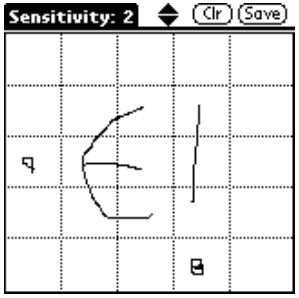
\includegraphics[width=0.3\linewidth]{rw/draw-a-secret}
		\caption{\label{fig:rw:drawmetric}}
	\end{figure}
	
	However, once unlock on Android had become a standard authentication technique for millions of users, a number of formal evaluations were carried out by the academic community. Harbach \etal pointed out that participants in their longitudinal study spent around 2.8 minutes on average per day to unlock their phone \cite{Harbach2016HardLockLife}. Interestingly, patterns were entered significantly faster than traditional PINs on average. 
	% attacks: smudge
	Regarding their proneness to attacks, it was recognized early that grid-based patterns on a touchscreen are also prone to ``smudge attacks'' where attackers can restore the user's pattern by looking at the oily residue left on touchscreens after entering the pattern \cite{Aviv2010SmudgeAttacks}. 
	% attacks: shoulder surfing: 
	De Luca \etal conceived an approach to authenticate on the back of smartphones and iterated the concept \cite{DeLuca2013BackOfDevice,DeLuca2014NowYouSeeMe}. Authenticating on the back has the big advantage to be resilient against shoulder-surfing attacks. Von Zezschwitz \etal also investigated which specific pattern types were most resilient to shoulder-surfing even if the attacker can observe them directly \cite{VonZezschwitz2015EasyToDraw}. Since the pattern unlock on Android cannot include a given dot multiple times, Colley \etal extended it that way \cite{Colley2016ExtendingPatterns}. This approach effectively thwarts smudge attacks with a minimal change to the existing system. 
	% predictability.
	Moreover, Uellenbeck \etal \cite{Uellenbeck2013QuantifyingSecurityPatterns}, as well as Von Zezschwitz \etal \cite{VonZezschwitz2016QuantifyingEffective} quantified the effective pattern space. Both their conclusion was that user-chosen patterns are very predictable, so the hypothesized security benefits of patterns over PINs are questionable. At the same time, Von Zezschwitz \etal tried to nudge users to pick a less predictable starting position with different types of background images \cite{VonZezschwitz2016QuantifyingEffective}. Their approach resembled Background-Draw-a-Secret (BDAS) \cite{Dunphy2007BDAS} and Persuasive Cued Click Points (PCCP) \cite{Chiasson2008PCCP}. When evaluating the concept through an online study, the effects on user selected patterns, however, remained small.

	\paragraph{Summary and Future Directions}
	% maybe we understand too little.
	Apart from the pattern unlock for on Android, graphical authentication systems have not been adopted widely. Text-passwords are still the preferred option for many service providers and are still available as authentication method on mobile devices. Maybe, we need to improve understanding as to why the supposed advantages of greater memorability and security have not been able to outweigh the disadvantages (authentication times, shoulder surfing). As of know, little is known about the mental models of graphical password security. A step in this direction was Katsini \etal's recent work \cite{Katsini2017StrategiesGraphicalPasswords}. They explored mental models and strategies that users employ to create graphical passwords. Thorpe \etal also found out that there are presentation effects that influence how people pick graphical passwords \cite{Thorpe2014PresentationEffects}. 
	
	% where to go from here. 
	For the future, we could narrow down the most feasible direction for visual authentication \cite{Biddle2009GraphicalFirstTwelveYears}. To get there, Stobert and Biddle compared searchmetric, locimetric and drawmetric systems in terms of password memorability \cite{Stobert2013GraphicalPasswords}. All participants in their study were assigned a system-generated password to reduce biases. Unsurprisingly, recognition based systems performed better than recall based systems (``recognition rather than recall is one of the most important usability heuristics \cite{Nielsen1994EnhancingHeuristics}). Nonetheless, this seems to be the most feasible approach that might see new ideas in the near future.
	% critics
	However, De Angeli and Renaud \etal doubt that visual authentication methods will prevail ub the long run \cite{DeAngeli2005PictureThousandWords, Renaud2009VisualSnakeOil}. They argue that the promise of more memorable passwords has not been fulfilled by the approaches so far and that we should keep looking elsewhere. Potentially, we will rely on less knowledge-based authentication in the future, but more on biometric and multimodal approaches. Those are discussed in the following. 

	\subsection{Biometrics and Multimodal Authentication}
	% leaving knowledge-based authentication at this point
	% now: something that you are or that you do
	Recent market analyses indicate that over 70\% of smartphones will ship with a fingerprint sensor in 2018 \footurl{https://www.counterpointresearch.com/more-than-one-billion-smartphones-with-fingerprint-sensors-will-be-shipped-in-2018/}{02.01.2018}. Those biometric sensors are most commonly used for user identification and authentication. In this section we take a brief look at the different features that can be used in biometric authentication, the advantages of combining them, and where they can fail. 
	
	For biometric authentication, there exist two common categories: \textit{Explicit} and \textit{implicit} authentication. In an explicit authentication scheme, the user is prompted to provide the proof of identity, e.g. the fingerprint. The idea behind implicit authentication, as Jakobsson \etal describe it, is essentially to ``authenticate mobile users based on actions they would carry out anyway'' \cite{Jakobsson2009ImplicitAuthentication}. For example, walking, typing, or simply using the device in a specific environment.
	
	% biometric features that are used for authentication
	\subsubsection{Explicit Biometrics}
	\textbf{Fingerprints} are becoming\footurl{https://www.deloitte.co.uk/mobileuk/\#gold-finger-fingerprints-lead-biometric-authentication}{02.01.2018} the most common feature used biometric authentication method nowadays, due to the widespread device-support (mobile phones, tablets, laptops) and obvious usability benefits as perceived by the users\cite{Wash2010FolkModels}. On modern phones, after a short enrollment, fingerprint recognition takes a fraction of a second and has low error rates under normal circumstances \cite{Henniger2016SecurityEvaluationFingerprint}. 
	% examplary problems
	Thus, fingerprint authentication is fairly usable and reasonably secure. However, a wet surface, grease, or dirt can limit the functionality \cite{Bhagavatula2015BiometricPerceptions}. 
	% attacks
	Moreover, there are different kinds of attacks if the victim is not in the vicinity (like fingerprint spoofing with a 2D/3D print). Such attacks are becoming easier to carry out, though they still require decent effort \cite{Marasco2014SurveyAntispoofing}. But if, for example, the victim is asleep, it is enough to hold the finger onto the sensor to gain access to the device (which can indeed cause relationship fights that can force airplanes to land early\footurl{https://www.theguardian.com/world/2017/nov/08/qatar-airways-plane-forced-to-land-after-wife-discovers-husbands-affair-midflight}{28.12.2017}).
	
	% IRIS AND FACE
	Recently, more systems are counting on \textbf{iris and facial recognition} to authenticate users. Windows Hello is a framework for biometric authentication that includes not only fingerprint support, but also authenticates users through their iris or face\footurl{https://support.microsoft.com/en-us/help/17215/windows-10-what-is-hello}{03.01.2018}. Mobile phones usually have a front-camera facing the user, so Android has included the ``Face-Unlock'' feature since version 4 (2011), which was rebranded to ``Trusted Face'' in version 5 (2014)\footurl{https://www.androidcentral.com/smart-lock-screen-security-options-android-50-lollipop}{03.01.2018}. Moreover, on the iPhone X (2017), Apple has removed the home button and with it the fingerprint reader and the TouchID system in favor of FaceID\footurl{https://support.apple.com/en-us/HT208108}{03.01.2018}. With FaceID, the user simple picks up the phone and looks at it to unlock it. The chance of another person unlocking the phone the same way is 1 to 1 Million, according to Apple. 
	% attacks
	However, it is possible to fool face-unlock systems with different spoofing attacks like using a face mask\footurl{https://www.theverge.com/2017/11/13/16642690/bkav-iphone-x-faceid-mask}{03.01.2018}, or in some cases a simple image of the legimitate user. All the aforementioned systems use a PIN/Passcode as fallback method that dominates the biometric schemes. 
	% HCI Studies
	De Luca \etal evaluated the reasons for (not) using biometric authentication on mobile devices in an online survey \cite{DeLuca2015Selfies}. They found that users prioritize usability over security when deciding which unlock mechanism to use. The respondents who had deactivated Face Unlock mostly did so for usability (read: interaction times) and reliability reasons. Interestingly, most respondents were aware of the security trade-off that face recognition entails.
	
	% VOICE
	Finally, a last example for explicit biometric authentication is \textbf{voice recognition} \cite{Aleksic2006AVBiometrics}. Android and Google Home appear to be the only consumer-oriented systems that allow users to authenticate through their voice \ar. Hang \etal evaluated a password reset system that uses voice recognition to verify the reset request \cite{Hang2013TravelRoutes}. They point out the importance to consider embarrassment in the design of natural voice interaction, e.g. in an office environment. Moreover, ``Both face and voice recognition logins are extremely situational dependent; [...] speaking into a microphone doesn't always work in noisy environments''\footurl{https://www.inauth.com/blog/fingerprints-popular-biometric/}{02.01.2018}, so it is important to create systems that adapt to contexts \cite{Damousis2008Humabio}.
	
	% features that are used for implicit authentication
	\subsubsection{Implicit Biometrics}
	Implicit authentication is done without prompting or challenging the user, but to continuously verify his or her identity \cite{Peisert2013PriciplesAuthentication}. One goal is to achieve a more natural interaction, similar to human-human interaction. Greenstadt and Beal postulate a system that recognizes people like humans do: ``in most everyday interactions, we recognize people by who they are and how they behave, rather than by the secrets that they know'' \cite{Greenstadt2008CognitiveSecurity}. Of course, this excludes situations where two strangers need to authenticate one another, e.g. at a passport control at the border. A specific key benefit of successful implicit authentication would be that users do not have to spend time authenticating explicitly, which can save them a couple of minutes per day \cite{Harbach2016HardLockLife}. 
	
	% GAIT
	The way a person walks is one of the features that can be used to recognize them, which humans can easily do \cite{Cutting1977GaitPerception}. One of the early approaches to exploit gait patterns for authentication can be traced back to Ailisto \etal who equipped laptop computers with accelerometers \cite{Ailisto2005GaitPatternAccelerometers}. They achieved to identify users this way with an EER of 6.5\%.  Tamviruzzaman \etal implemented this approach for mobile phones that at the time (2009) had started to integrate acceleration sensors and gyroscopes \cite{Tamviruzzaman2009ePet}. For their ``ePet'' system, they also combined gait patterns with GPS-location traces, but did not report on a user study. Muaaz and Mayrhofer tackled the issue of device orientation and achieved an EER of 7.05\% in the same study session, but only 18.96\% across multiple sessions. As of now, gait recognition has not been widely adopted, but Android allows the user to activate ``on body detection'', which keeps the device unlocked while it is in motion\footurl{https://support.google.com/nexus/answer/6093922?hl=en}{03.01.2018}. Reportedly, ``some devices'' can learn the gait pattern and lock the device if they detect a different walking style. As shown in Table \ref{tbl:rw:auth_comparison}, gait detection faces a number of problems which are difficult to overcome. 
	
	
	% INTERACTIONS WITH DEVICES: KEYSTROKES / GESTURES
	Another theme in implicit authentication is \textit{behavioral} biometrics. For instance, the way people use their mobile phones and in which contexts can be used to build a user model \cite{Jakobsson2009ImplicitAuthentication}. Keystroke dynamics, i.e., characteristic typing patterns, can also serve as feature. The first algorithms were conceived for desktop environments \cite{Crawford2010KeystrokeDynamics}, but Bouchoux and Clarke proposed an early solution in 2008 that achieves authentication via keystrokes on smartphones \cite{Buchoux2008KeystrokeAnalysis}. They state that explicitly enrolling users might be too bothersome for them, so it should be possible to enroll a user implicitly. This in turn produces a risk of including data from impostors, too. De Luca showed that users enter grid-based patterns in a unique way, which can be leveraged for implicit authentication \cite{DeLuca2012TouchMeOnce}. Their second user study focused on this type of unlock mechanism and, with an average accuracy above 90\%, they could decide whether a correctly entered pattern was actually entered by the legitimate user. Interestingly, at the time of writing this thesis, De Luca \etal's paper is the most-cited CHI publication in the past five  years\footurl{https://scholar.google.com/citations?hl=en\&vq=eng_humancomputerinteraction\&view_op=list_hcore\&venue=6NNnGOq9_mAJ.2017}{03.01.2018}, which highlights the impact and potential of this approach. What is more, this is the one of the few approaches that makes explicit authentication more secure through a second, biometric layer. While the user models of the aforementioned approaches are created and maintained on the devices, Nauman and Ali proposed a system architecture that shifts keystroke analysis to a Trusted Third Party, which authenticates the user \cite{Nauman2010TOKEN}. However, their approach requires more sophisticated hardware (trusted platform modules), which renders it more costly.

	% SUMMARY and OUTLOOK
	\subsubsection{Summary and Outlook}
	Since all biometric features, if considered independently, can be spoofed in some way (see Table \ref{tbl:rw:auth_comparison}), approaches to combine multiple features have started to proliferate. Although the idea of \textit{multimodal} signals for authentication is not particularly new (some implementations were done in the mid 1990s \cite{Brunelli1995PersonIdentificationMultipleCues}), perhaps the computing power both on the clients and back-ends is now large enough to handle the input streams. Bigun \etal developed a framework that continues to learn from multiple signals \cite{Bigun2005CombiningBiometricEvidence}, which requires such computing power.	Rybinicek \etal presented a roadmap with obstacles and opportunities \cite{Rybnicek2014RoadmapContinuousAuth} that can serve the design of future multimodal biometric authentication schemes. Google, among other companies, tries to incorporate the notion of such multimodal implicit authentication in their Smart Lock solution\footurl{https://get.google.com/smartlock/}{03.01.2018}. 
	
	In summary, we can take away that biometric authentication provides many usability benefits like reduced time spent on authentication and also security enhancements. Though implicit authentication is unlikely to replace explicit authentication completely, it can still make explicit schemes more secure as demonstrated by De Luca \etal \cite{DeLuca2012TouchMeOnce}. In Section \ref{sec:rw:pws_are_here_to_stay}, however, we discuss why biometrics are still dominated by knowledge based authentication especially in situations where the system cannot make a final decision due to low certainty. 
	
	%%%%%%%%%%%%%%%%%%%%%%%%%%%%%%%%%%%%%%%%%%%%%%%%%%%%%%%%%%%%%%%%%%%%%%%%%%%%%%%%%%%%%
	%		Table: Biometric features overview											%
	%																					%
	%%%%%%%%%%%%%%%%%%%%%%%%%%%%%%%%%%%%%%%%%%%%%%%%%%%%%%%%%%%%%%%%%%%%%%%%%%%%%%%%%%%%%
	\begin{table}[htbp]

\rowcolors{2}{AliceBlue}{Beige}
\centering
\resizebox{\linewidth}{!}{
\begin{tabular}{|m{3cm}|m{3cm}|m{3cm}|m{3cm}|m{3cm}|} \hline
\textbf{Feature}&\textbf{Capturing Method}&\textbf{Implicit / Explicit}&\textbf{Spoofing Threats}&\textbf{Problems}\\ \hline \hline

Face \& Iris & Camera & Both & Photographs of the legitimate user & Lighting situation and make-up  \\ \hline

Fingerprint & Fingerprint reader & Explicit. Implicit imminent. & Play-Doh casts, Scotch Tape, 2D/3D prints  & Dirt, Water, Finger injuries \\ \hline

Speech & Microphone & Both & Recordings of the user's voice & Sickness, natural voice changes, background noise \\ \hline

Gait	 & Camera or Accelerometer & Both & Imitation  & Injuries, carrying load, footwear, ground surface, being seated \\ \hline

Keystroke & Hard/soft keyboard & Primarily implicit & Imitation & Enrollment, reliability \\ \hline

Location & GPS or infrastructure calculated position & Primarily implicit & Forged GPS locations & limited places, precision \\ \hline

Network/File/App Usage & Software protocol & Implicit & Imitation & Precision \\ \hline

%Call Patterns & Log Data & implicit & None & No constraints & high efficacy variance for different users \\ \hline

\end{tabular}
}
\caption{\label{tbl:rw:auth_comparison}Comparison of different biometric authentication methods}
\end{table}
		
	\subsection{Multi-Factor, Token-based and Federated Authentication}\label{sec:rw:shared_auth_tokens}
	As a final aspect of authentication beyond passwords, let us take a look at systems that do not necessarily aim to replace passwords, but to make them more user-friendly and/or secure. 
	
	\paragraph{Two-Factor Authentication}
	% multifactor authentication: description and everyday example
	In a multi-factor authentication, the user needs to present multiple credentials to the systems in whichever form. For instance, the Google 2-step verification mechanism combines the user-chosen password with a \textit{one-time password} (OTP)\footurl{https://www.google.com/landing/2step/}{04.01.2018}. For instance, if users log into their Google account on a computer in an Internet café, they will receive an OTP on a secondary device, usually in a text message sent to their personal phone. If no more than two separate channels (``\textit{out of band authentication}'', OOBA) are involved, the scheme is usually referred to as Two-factor authentication or 2FA for short. Multi-factor authentication aims to prevent impersonation in case an attacker has obtained a victims primary credential, but not their secondary factor. 
	% early work / ideas
	There were hints to combining multiple such levels to make authentication more robust already in the late 1970s. Morris and Thompson mentioned that ``some UNIX systems have instituted what is called an `external security code' that must be typed when dialing into the system, but before logging in. If this code is changed periodically, then someone with an old password will likely be prevented from using it [the system, author's note]'' \cite{Morris1979PasswordSecurity}. Moreover, in 1984 Haskett shared an idea about a second level of authentication in 1984 \cite{Haskett1984PassAlgorithms}. With the \textit{Pass-Algorithms} mechanism, the user first authenticates with their regular credentials and then proves their identity by responding to a random prompt by completing a pre-shared procedure. The algorithm is altered by the system administrator and then shared with the legitimate users, who are supposed to memorize the algorithm rather than a static password. For instance, the current algorithm could be to use the subsequent letter in the alphabet based on the challenge: If the challenge is BEL, the user enters CFM as second layer of authentication. The proposed benefit is that the algorithm is easier to remember and can still be personalized. 
	% MFA nowadays, tradeoffs.
	Multi-factor authentication has since been widely adopted and more web services are following. Many banks have the users confirm transactions by a transaction number (TAN) sent to their phones, although they are already logged in with their banking password \cite{Maurer2011DataTypeWarnings}. The primary benefit of multi-factor authentication lies in the increased confidence of the legitimacy of account actions. In any case, there is a small usability caveat, because adding more factors leads to longer interactions, which is not recommendable for secondary tasks like authentication \cite{Adams1999UsersEnemy}. However, the increased security might in turn improve user experience because it also empowers users to be certain about interacting with the legitimate party. Attacks on multi-factor authentication are possible\footurl{https://www.theverge.com/2017/9/18/16328172/sms-two-factor-authentication-hack-password-bitcoin}{04.01.2018}, but do not scale well \cite{Herley2014CybercrimeAtScale}.
	
	% ONE TIME PASSWORDS
	Moreover, one-time passwords and ``Magic Login Links''\footurl{https://www.sitepoint.com/lets-kill-the-password-magic-login-links-to-the-rescue/}{04.01.2018} can also replace user-chosen passwords \todo{a graphic would be nice to illustrate how this works}. The user only provides their user name, and the system sends them a magic link or a random one-time password to their verified email account or phone. So, in that sense, accessing one's personal email account is the primary authentication factor. After clicking the link or logging in with the OTP, the link or OTP expires. If implemented at scale, this could allow users to only memorize the credentials for their email account and log in to all other systems by receiving magic links. However, the approach is only secure under the assumption that the email account is well protected. It might be fair to assume that users might underestimate the risk of relying on magic links. For low-value accounts, though it seems like a viable and promising solution although trust issues on the user side need to be further addressed \cite{Ruoti2015AuthenticationMelee}.  
	
	\paragraph{Hardware Tokens and Proxies}
	Hardware tokens are often a special flavor of multi-factor authentication, but it is worthwhile to treat them separately, because in some cases they can act as standalone replacement of passwords, too. In general, this solution uses a hardware device to store user secrets \cite{Bonneau2012ReplacePasswords}. In multi-factor environments, the RSA SecurID token\footurl{https://www.rsa.com/en-us/products/rsa-securid-suite/rsa-securid-access/securid-hardware-tokens}{04.01.2018} displays a random numerical which is valid for at most 60 seconds, and the user has to enter it as second factor. The YubiKey tokens\footurl{https://www.yubico.com/start/}{04.01.2018} are inserted into the USB port of the computer or held against an NFC-equipped smartphone to prove the user's identity (see Figure \ref{fig:rw:hardware_tokens}). While the two device improve account protection, the downside is that they are easily lost or stolen, and have to be with the user when they wish to authenticate. 
	
	% wearable tokens: 
	To save users from entering PINs, patterns, or passwords to unlock their phones, Jakobsson developed a bracelet that serves as secure token \cite{Jakobsson2014HowToWearYourPW}, which is not as easily lost or stolen. This idea is also embraced in commercial products. Smart watches and other wearables can serve as authentication tokens: Google offers the ``Trusted Device'' feature since Android version 5. If a trusted device, e.g. a smart watch or wireless headphones, is connected to the phone via Bluetooth, the phone turns off the primary authentication method, e.g. pattern unlock while the device is connected. If the phone has been inactive for four hours or had been manually locked, the user needs to re-authenticate by providing the primary credential. This can drastically reduce the number of authentication events, given phones are unlocked between 27 and 86 times per day by recent estimates\cite{Deloitte2017ConsumerSurveyUS, Stachl2017PersonalitySmartphones}. 
	
	\begin{figure}[htbp]
		\centering
		\begin{subfigure}[t]{0.49\linewidth}
			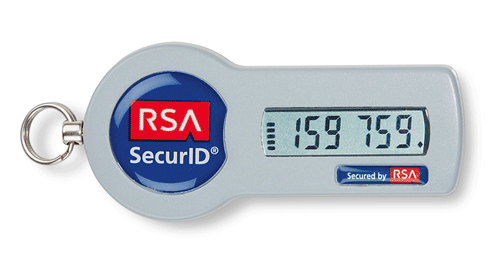
\includegraphics[width=\textwidth]{rw/securid-token}
			\caption{The RSA SecurID token displays a one-time-password every 30 to 60 seconds}
		\end{subfigure}
		\begin{subfigure}[t]{0.49\linewidth}
			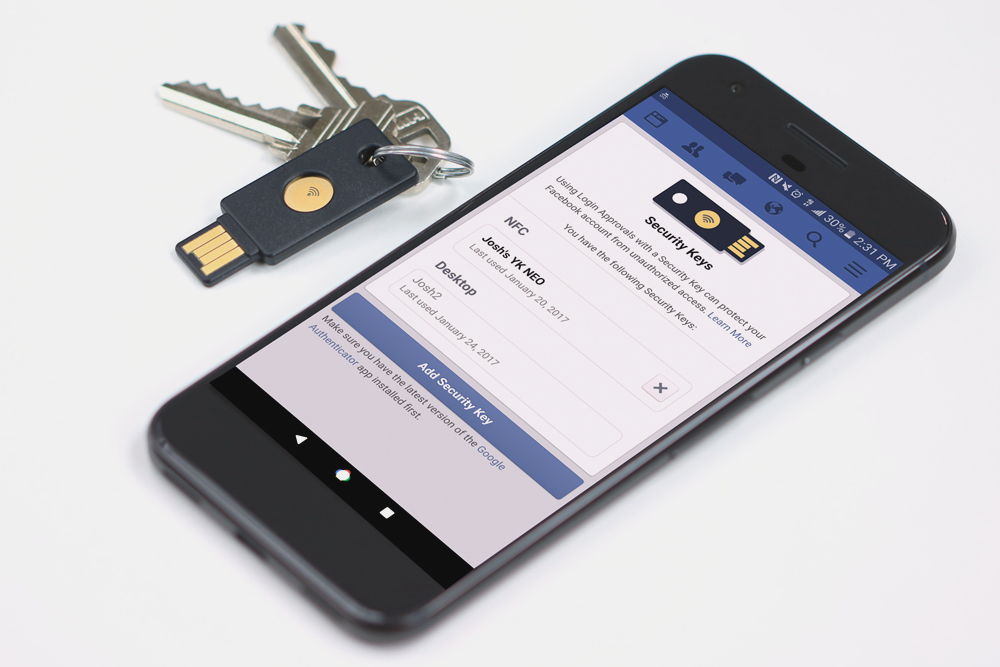
\includegraphics[width=\textwidth]{rw/yubiey-facebook-login}
			\caption{YubiKey uses NFC to authenticate users.}
		\end{subfigure}
		\caption{\label{fig:rw:hardware_tokens} Commercially available hardware tokens. The RSA SecurID is more business-oriented, while the YubiKeys can be used with consumer products like Gmail, Facebook, and Dropbox, too.}
	\end{figure}
	
	Other approaches leverage devices that the users carry with them anyhow as authentication token or proxy. Aebisher \etal present the Pico Framework where the user has to scan a QR code with a special app to pass-by manual authentication \cite{Aebischer2017PicoInTheWild}. Some banks require the user to scan special image codes as second factor during authentication\footurl{http://www.wikibanking.net/onlinebanking/verfahren/phototan/}{04.01.2018}. A few popular websites have already started to adopt the system. Roalter \etal presented a system that allowed users to access shared rooms in a university by authenticating with their smartphone \cite{Roalter2013SmartphoneProxy}. There is some evidence that users generally appreciate this kind of interaction \cite{Ruoti2015AuthenticationMelee}. However, using the phone as proxy or second factor has the disadvantage that batteries might be empty when or the phone was stolen. 
	
	\paragraph{Federated Single Sign On}
	The idea behind single-sign on (SSO) is to allow the user to log into one service and other services can use this login state without requiring any more explicit authentication actions. Thus, the user must only remember one set of credentials \cite{Egelman2013ProfilePassword}. With federated single sign-on, websites can authenticate users by temporarily redirecting them to a trusted third party \cite{Bonneau2012ReplacePasswords}. The third party verifies the user's identity. Afterwards it signs the authentication request and returns a text-based token that the client needs to present in future interactions. A historically successful example is Kerberos \cite{Kohl1993Kerberos}. However, SSO approaches did not receive widespread acceptance for about twenty years \cite{Sun2010BillionKeys}. Currently, the OpenID protocol is a state of the art approach, where user identities are verified in a decentralized approach \cite{Recordon2006OpenID}. Any web server can act as identity provider, but it is most feasible if trustworthy parties enable OpenID. Currently, Microsoft, Google and Oracle are among the biggest OpenID identity providers. \textbf{OAuth} is a related protocol, but is not designed as identity proof but to allow ``relying parties'' to use resources on other websites \cite{Bonneau2012ReplacePasswords}. For example, a web app can use OAuth to access profile information on Facebook or publish Twitter messages on the user's behalf. The web app can create a separate user-account with the data it receives from the OAuth interfaces, and automatically authenticate the user without further notice. Perhaps this is the reason OAuth is often mistakenly seen as single-sign-on mechanism. 
	
	Different analyses of the security and user experience of SSO mechanisms have yielded mixed results. Ruoti \etal found that their participants ranked OpenID-like approaches as preferred way to authenticate \cite{Ruoti2015AuthenticationMelee}. Sun \etal, however, found that their survey respondents had often erroneous mental models about how single-sign on works \cite{Sun2011UsersRefuseSSO}. For instance, many people thought that their passwords are shared with relying parties and also around 40\% were concerned about privacy in this study.  Contrarily, Egelman pointed out that users who used Facebook Connect are fairly cognizant of the data that is shared with relying parties \cite{Egelman2013ProfilePassword}. Still, 15\% of respondents expressed privacy concerns and refrained from using such mechanisms. Bonneau \etal also criticize big companies as identity providers by noting that ``Facebook Connect (a version of OAuth), incentivizes relying parties with user data, mandating a central role for Facebook as the sole identity provider, which does little for privacy'' \cite{Bonneau2015ImperfectAuthentication}.	For users, leaving an identity provider like Facebook also entails tedious account recovery on relying services like Spotify\footurl{https://tobiasseitz.wordpress.com/2016/12/20/how-to-use-spotify-after-leaving-facebook/}{04.01.2018}.In summary, SSO theoretically has the potential to drastically reduce the number passwords but it brings out a new range of problems. 

\subsection{Passwords are Here to Stay}\label{sec:rw:pws_are_here_to_stay}
% this doesn#t have to be super long but it should highlight the key aspects where alternative solutions fail to replace passwords.
Most of the solutions we discussed in Sections \ref{sec:rw:graphical_pws} through \ref{sec:rw:shared_auth_tokens} could theoretically abolish the need for users to create, manage and live with passwords entirely. Many of them have existed for decades -- visual authentication, biometrics and federated approaches all have their roots in the 1990s. Biometric authentication has been widely adopted and commercially successful since smartphones have proliferated and become an indispensable part for many people's day-to-day activities. Some analysts even predict that in 2020, all mobile devices will be equipped with biometric sensors to authenticate users\footurl{https://www.enterprisemobilityexchange.com/news/fast-facts-all-mobile-devices-will-use-biometrics}{11.01.2018}. Modern versions of OAuth/OpenID as well as authentication-as-a-service (AAAS) solutions make it exceptionally easy to avoid the costs of setting up infrastructures for the simple task of authenticating users -- a well-defined task since the 1960s. Still, we use passwords basically every day. So why has it not been possible to replace passwords? Bonneau \etal provide us with an evaluation framework for web authentication schemes \cite{Bonneau2012ReplacePasswords}. In there, they identify three major aspects where alternative solutions can fall behind passwords: Usability, deployability, and security. In the following, we summarize the central issues with the most likely candidates to replace passwords, biometrics and SSO. The argumentation is inspired by Bonneau \etal's work, but extended by a few notable aspects that have become important since they published their paper in 2012. 

\paragraph{Usability}
As we discuss in Chapter \ref{chap:rw:user_perspective}, the usability of passwords is generally seen as low, mostly because they take long to enter and it is tedious to memorize them. Especially on mobile devices which are ever more used, this drawback gains weight. But still, the system is easy to learn and users mostly have it in their own hands to reset passwords. ``Muscle-memory'' reduces the cognitive effort to recall passwords. 
Biometrics seem to trump passwords in the usability dimension, because it is very convenient to authenticate with biometric features. However, there is one fatal showstopper. It is impossible to manually reset, e.g., a fingerprint after it has been compromised. It is difficult to communicate to users where their data is stored and that attacks are unlikely. Moreover, a biometric system makes fuzzy instead of binary decisions. Thus, in many cases the required probability thresholds are not met and this bad reliability of sensors and algorithms leads to user frustration. Sharing accounts that are protected with biometrics also require more elaborate architectures and cumbersome setup. Finally, all biometric systems have fallback mechanisms, that more often than not rely on passwords, which leads to new usability problems. SSO also gives users more ease of use, especially because it reduces the cognitive effort required to authenticate. Still, people's trust issues as well as sub-par mental models appear to outweigh the usability benefits. Another large usability drawback is the strong lock-in effects established by identity providers. In summary, both biometrics and federated authentication face insurmountable usability hurdles. 

% costs / deployability
\paragraph{Deployability} 
Regarding deployability, and thus setup costs, nothing seems to beat passwords. With a plethora of web-authentication frameworks for different platforms, production-level authentication workflow can probably be set up in less than a day. It is possible to build user interfaces for password-based authentication on virtually all systems that take alphanumeric user input. Biometrics often require hardware sensors, or in the case of behavioral biometrics a powerful back-end suitable for deep learning and handling massive data streams. It is infeasible to build a fingerprint or iris reader into a Smart TV, for example. The know-how required to set up artificial intelligence utilized for authentication has become smaller with the advent of frameworks like Tensorflow, but it is anything but trivial to do it right on a larger scale. SSO is probably easier to deploy than biometrics, because there is a negligible cost per user. Frameworks also facilitate set up. However, switching to SSO can lead to incompatibilities with existing schemes which increases costs for transition phases and hybrid approaches. In conclusion, passwords are unbeatable in terms of deployability and the costs it entails to set up password-based authentication. 

% security
\paragraph{Security}
As discussed in Section \ref{sec:rw:attack_vectors}, we can safely assume that if an attacker is dedicated enough to compromise a password-protected system, they will probably succeed to some degree (depending on the scale of the attack). Security-wise, biometrics do not really outperform passwords apart from the uniqueness of the ``secret'' and physical observability. However, not only do we leave our fingerprints in many public places, but also do we have to acknowledge that a user's fingerprint is translated into a digital ``file'', which can leak. Detecting this attack is more troublesome than for passwords: A simple Internet search can help users in finding out whether their password has leaked, but searching for a leaked fingerprint, let alone other biometric user models, complicates this effort a lot. SSO does in fact provide more security benefits over passwords than biometrics. The risk of credential spillage is minimized, and the attack surface for guessing and observation attacks becomes smaller if only trusted identity providers take care of authentication. Then again, the responsibility that lies with identity providers is high. Instead of a more disperse attack landscape, there might be a concentration on these parties if SSO were to become the de facto standard.

	
%Matyás and Riha pointed out the advantages and disadvantages of biometric systems in general \cite{Matyas2003ReliableUserAuthentication}
% since probability != certaint: biometrics need a fallback strategy
%It is an important key feature of biometric authentication that the result is non-binary and involves a predefined threshold that defines when the provided information looks ``legitimate enough'' to authenticate the user. To account for the lack of certainty, in all current state-of-the-art mechanisms passwords serve as fallback authentication. So, while it reduces the number of password entries and speeds up interactions in many cases, these schemes cannot fully replace passwords. What is worse is that the rare interaction often tempts users to choose a very memorable fallback secret \cite{Cherapau2015ImpactOfTouchID}, which in most cases is weaker than a password that is entered on a regular basis. So in a scenario in which the system successfully locks out an attacker, they will always have the opportunity to authenticate with the fallback method, because the system needs cannot fully exclude a false rejection. In this scenario, while the primary authentication is more usable and very secure, the entire system's security is lowered by its fallback scheme.  

\paragraph{Conclusion: Passwords are not going away, just yet.}
Bonneau \etal argue that passwords are an imperfect technology that is difficult to replace and so they answer the question as to if we still need passwords with a differentiated ``yes'': \textit{``Passwords appear to be a Pareto equilibrium''}\footnote{By equillibrium, the authors most likely mean a Pareto efficient state. From WikiPedia: ``Pareto efficiency or Pareto optimality is a state of allocation of resources from which it is impossible to reallocate so as to make any one individual or preference criterion better off without making at least one individual or preference criterion worse off.'' \url{https://en.wikipedia.org/wiki/Pareto_efficiency}, \textit{last accessed 04.01.2018}} \cite{Bonneau2015ImperfectAuthentication}. The industry has found ways to work around the drawbacks that passwords certainly entail. Thus, if passwords are not going away, multi-factor and multi-modal systems may turn out to be the most promising solution. The challenge is to establish a minimally privacy-sensitive solution that embraces user-centered design to a higher degree than previous multi-factor/-modal approaches. Academic research can, according to Bonneau \etal, carry out experiments that would potentially have a detrimental effect on business successes and thus help in pushing viable solutions forward. As Herley and van Oorshot point out: ``[...] it is time to admit that passwords will be with us for some time, and moreover, that in many instances they are the best-fit among currently known solutions.'' \cite{Herley2012PersistenceOfPasswords}. They propagate a more systematic approach to make users' lives easier instead of trying to find the single panacea that replaces passwords entirely.

%\cite{Kirlappos2012SecurityEducation,Loutfi2015PasswordsOtherSideOfTheFence,DeAngeli2005PictureThousandWords,Florencio2013WhereDoAllTheAttacksGo,Herley2008ProfitlessEndeavor,Sasse2015,Dittrich2009,Herley2009SoLongThanksExternalities,Vantaggiato2015WeStillNeedPasswords,Florencio2010WhereDoPoliciesComeFrom,Schrittwieser2013,Bonneau2015ImperfectAuthentication,Cyber2014,Florencio2007DoStrongWebPasswords,Sasse2005UsableSecurityPosition,Aebischer2017PicoInTheWild,Forget2007HelpingUsers,Herley2009IfWereSoSmart,Acar2016NotYourDeveloper,Sasse2016,Renaud2009VisualSnakeOil}

 